\documentclass[11pt]{article}
\usepackage{amsfonts,amsmath,amssymb,amsthm}
\usepackage{graphicx,psfrag,epsf}
\usepackage{enumerate}
\usepackage{url} % not crucial - just used below for the URL 
\usepackage{algorithm}
\usepackage{algpseudocode}
\usepackage{subfig}
\usepackage{authblk}
\usepackage{verbatim} %used to comment out unnecessary contents
\usepackage{helvet}
\usepackage[colorlinks=true,pagebackref,linkcolor=magenta]{hyperref}
\usepackage[sort&compress,comma,square,numbers]{natbib}
\usepackage{fullpage,fancyhdr}
\renewcommand{\familydefault}{\sfdefault}
\usepackage{color} %used to highlight changes

%\pdfminorversion=4
% NOTE: To produce blinded version, replace "0" with "1" below.
\newcommand{\blind}{0}

% % DON'T change margins - should be 1 inch all around.
% \addtolength{\oddsidemargin}{-.5in}%
% \addtolength{\evensidemargin}{-.5in}%
% \addtolength{\textwidth}{1in}%
% \addtolength{\textheight}{-.3in}%
% \addtolength{\topmargin}{-.8in}%


\pagestyle{fancy}
% \oddsidemargin=-0.5in 
% \evensidemargin=-0.5in
\textwidth=6.5in 
\headwidth=6.5in
\textheight=9.0in 
\headheight=0.0pt
\topmargin=0.0in
\headsep=0.0in
\renewcommand{\headrulewidth}{0pt}

\setlength{\parindent}{0em}
\setlength{\parskip}{0.5em}


\providecommand{\mt}[1]{\widetilde{#1}}
\providecommand{\mb}[1]{\boldsymbol{#1}}
\providecommand{\mc}[1]{\mathcal{#1}}
\newcommand{\Real}{\mathbb{R}}


%environment
\newtheorem{thm}{Theorem}
\newtheorem{lem}{Lemma}
\newtheorem{cor}{Corollary}
\newtheorem*{defi*}{Properties}
\newtheorem{asn}{Assumption}
\newcommand*\mean[1]{\bar{#1}}
%\newproof{proof}{Proof}
%\newproof{proof}{Proof}
\begin{document}

\def\spacingset#1{\renewcommand{\baselinestretch}%
{#1}\small\normalsize} \spacingset{1}

\title{\bf Dependence Discovery across Scales from Multimodal Data via Local Graph Correlation}
\author[1]{Cencheng Shen\thanks{cshen@temple.edu}}
\author[2]{Joshua T. Vogelstein\thanks{jovo@jhu.edu}}
\author[3]{Carey E. Priebe\thanks{cep@jhu.edu}}
\affil[1]{Department of Statistics, Temple University}
\affil[2]{Department of Biomedical Engineering,  Institute of Computational Medicine, Johns Hopkins University}
\affil[3]{Department of Applied Mathematics and Statistics, Johns Hopkins University}
\maketitle
\pagestyle{empty}

\bigskip
\begin{abstract}
Understanding and discovering dependence between multiple properties or measurements of our world is a fundamental task not just in science, but also policy, commerce, and other domains. In the past hundred years, people have developed many different measures of dependence that can be applied in a wide variety of settings.  An ideal dependence measure would have the following properties. (1) Strong theoretical support, guaranteeing rejecting independence no matter what the dependence structure is, and failing to reject when no dependence is present. (2) Strong empirical support on a wide variety of low- and high-dimensional simulation settings. (3) Provides insight into the local scale in which dependency is strongest. (4) On real data, detects dependence when it exists, and fails to detect dependence when it does not exist. No existing test satisfies all of these properties. We develop a novel dependence statistic and test called ``Local Graph Correlation'' (LGC).  Briefly, we combine the ideas of distance correlation testing with nearest-neighbor testing.  LGC has all four of the above properties, as demonstrated by extensive theory, simulations, and real data examples. We can therefore use this test in a variety of settings in which previous tests failed to detect signal or provide insight.

YYY is it a bit strong to say 'No existing test satisfies all of these properties' in the abstract, despite it is true? YYY
\end{abstract}

\noindent%
{\it Keywords: distance correlation, k-nearest-neighbor, independence test, permutation test}  
\vfill

\clearpage
\tableofcontents


\newpage
\spacingset{1.45}

\section{Introduction}
With the increasing type, size, and dimension of modern data sets, detecting dependency among multiple data sets is one of the most important and fundamental tasks in the big data age. The Pearson's correlation coefficient \cite{Pearson1895}, Spearman's and Kendall's rank correlation coefficient \cite{KendallBook}, RV coefficient \cite{RobertEscoufier1976}, Procrustes coefficient \cite{GowerProcrustesBook}, information theoretic measures \cite{Renyi1959}, and the Mantel test \cite{Mantel1967} have been the traditional tools for this task, but each has its limitations when dealing with the increasingly complex modern data sets, e.g., the Pearson's correlation coefficient and RV coefficient are mostly useful for finding linear relationship and may be zero for nonlinear dependent data sets, while mutual information performs poorly for high-dimensional data. 

Many recent methods have been proposed to identify the existence of potential relationships between data sets, including \cite{Baringhaus2004,TaskinenOjaRandles2005, GrettonEtAl2005, SzekelyRizzoBakirov2007, GrettonGyorfi2010,Reshef2011, HellerGorfine2013, Reimherr2013, SzekelyRizzo2013a, SzekelyRizzo2013b}, etc. In particular, the distance correlation method from \cite{SzekelyRizzoBakirov2007, SzekelyRizzo2009, SzekelyRizzo2013a, SzekelyRizzo2014} has gained much popularity in the statistical community, due to its theoretical soundness and good numerical performance in testing independence. A similar method from the machine learning point of view is the kernel-based independence test, which is developed in \cite{GrettonEtAl2005, GrettonGyorfi2010, GrettonEtAl2012}, and connected to the distance-based method in \cite{SejdinovicEtAl2013}.

Despite of current progress in the area, it remains a difficult problem to test dependency on real data; and even the best method in theory may suffer from one or more real challenges underlying the data, such as small sample size, high dimensionality, non-linearity, noise, etc. For example, although distance correlation is consistent against all dependent alternatives for testing on Euclidean data, the sample distance correlation (dcorr) under-performs in many high-dimensional or non-linear dependencies for finite-sample testing. The modified distance correlation (mcorr) from \cite{SzekelyRizzo2013a} adjusts the high-dimensional bias, but is still sub-optimal for many common non-linear dependencies. In comparison, the HHG statistic developed in \cite{HellerGorfine2013} performs much better on non-linear data of small sample size, but may lose some testing power for certain linear and high-dimensional dependency.

In a complementary literature, nearest-neighbor graphs have been used as a key computational primitive in many statistical approaches, ranging from classification and regression \cite{Stone1977} to data compression to recommender systems \cite{Sarwar2000}. 
More recently, nearest-neighbor has been an invaluable tool in unfolding nonlinear geometry in many recent development of nonlinear embedding algorithms, including Isomap \cite{TenenbaumSilvaLangford2000, SilvaTenenbaum2003}, Local Linear Embedding \cite{SaulRoweis2000, RoweisSaul2003}, and Laplacien eigenmaps \cite{BelkinNiyogi2003}, among many others. Furthermore, we have successfully applied joint neighborhood to unfold the non-linearity in multiple data sets in \cite{ShenVogelsteinPriebe2015}, which shows that a good choice of joint neighborhood can better match data sets of multiple modality. 



Most relevant to our work, a number of approaches to two-sample and dependence testing have utilized nearest-neighbor graphs \cite{David1966,Friedman1983,Schilling1986,Dumcke2014}.  These approaches have the advantage of naturally operating on any kind of data, including categorical and structured data, as well as strong theoretical guarantees.  Perhaps more importantly, they focus only on local distances, rather than global distances, enabling them to be robust to nonlinear and high-dimensional dependence structures.  However, none of the previous nearest-neighbor based methods provide a convenient or automatic method for choosing the neighborhood size, therefore leaving a crucial tuning parameter unspecified, and impairing its finite sample performance and practical usage. Moreover, they largely focused on two-sample testing, rather than dependence testing.  
YYY I am still not sure whether local distance enables robustness to hd dependency, since local dcorr is not robust to hd YYY

% Our local distance correlation shares a similar concept: by considering the inter-point distances limited to the $k$-nearest points, the local test statistic is naturally more informative than the global statistic for nonlinear dependency; while for close to linear dependency, the global statistic should still be the best.


In this paper we propose local graph correlation (LGC), in order to better address those challenges from modern data analysis. By marrying ideas from the distance correlation literature to those from the nearest neighbor literature, and adding some of our own special sauce, we obtain a test better than those in either camp.  More specifically,  the local test statistic naturally inherits the advantages of the distance correlation, such as being consistent, but also inherits properties of graph dependence structures, such as better performance in high-dimension and strongly nonlinear dependencies. In practice, LGC can be applied for testing dependence by the p-value from the permutation test; and the optimal neighborhood choice can be estimated by bootstrap, which is a standard resampling technique \cite{EfronTibshiraniBook}.

Those advantages make our new test statistic the best method thus far, for detecting dependency on complex simulated dependencies and real data. Indeed in our comprehensive simulation setting, local graph correlation is able to achieve a superior finite-sample testing power for data sets of non-linearity, noise, and/or small sample size, comparing to existing popular methods like dcorr/mcorr/Mantel/HHG; and in the real data experiment, LGC also returns the lowest p-value for testing dependency between human brain and human characteristics,  and will not detect false signals when the dependencies are not there in a set of brain imaging experiments. Thus, we expect LGC to find value in a wide range of applications.  To facilitate, we make all of our code open source and incorporate LGC into FlashR.
XXX still need to show this. XXX  
YYY send Jovo the data on YYY

% The paper is organized as follows: Section~\ref{main1} reviews the original distance correlation and the modified distance correlation. In Section~\ref{main2} we formulate the local distance correlation for both the original distance correlation and the modified distance correlation. Section~\ref{main3} discusses the evaluation procedure of testing independence, and in Section~\ref{main4} we show some theoretical advantages of local distance correlation. The simulation results are shown in Section~\ref{numer1} to demonstrate the numerical advantages of the local test statistic in various simulated relationships, and Section~\ref{numer2} illustrates its performance on real data sets. We conclude the paper in Section~\ref{conclu}, with proofs, additional propositions, and detailed simulation settings included in the appendix. The Matlab/R code for our method and the simulation is available on github\footnote{\url{https://github.com/jovo/Rankdcorr/}}. 

\section{Results}

\subsection{Intuition}

There are two key insights from the literature that we combine to develop our methodology.  First, a collection of pairwise comparisons  suffices to characterize a joint distribution \cite{Maa1996}.  Second, high-dimensional nonlinear manifolds can be approximated by local linear spaces.  Combining these two ideas yields our measure, the local graph correlation.  Perhaps the first realization that pairwise properties can characterize a joint distribution comes from  Karl Pearson, who created Pearson's Product-Moment Correlation \cite{Pearson1895}:
\begin{equation}
\label{generalCoef}
\frac{\sum_{i,j=1}^n a_{ij} b_{ij}}{\sqrt{\sum_{i,j=1}^n  a_{ij}^{2} \sum_{i,j=1}^n b_{ij}^{2}}}, 
\end{equation}

where $a_{ij}=x_i - \hat{E}(x_{i})$ (the expectation denotes the sample mean), and $b_{ij}$ is defined similarly for $y_i$.  Equation~\ref{generalCoef} can be treated as a general correlation coefficient, which characterizes most dependence measures since then.  For example, Spearman and Kendall's rank correlation let $a_{ij}$ equal $rank(x_i)-rank(x_j)$ and $sign(x_i-x_j)$, respectively \cite{KendallBook}; the Mantel coefficient \cite{Mantel1967} considers centered distances by letting $a_{ij}=|x_i-x_j|_{2}-\hat{E}(|x_i-x_j|_{2})$ (the expectation denotes the sample mean of all pairwise non-zero distances), which has been a popular method in biology and ecology. More recently, Szekely et al. \cite{SzekelyRizzoBakirov2007} lets $a_{ij}$ equal the doubly centered distances (so the matrix of $(a_{ij})$ has zero mean for each row and column), and show that their ``distance correlation'' statistic yielded a consistent test for dependency---a test whose power approaches $1$ as sample size approaches infinity---for any joint distribution of finite dimension and finite second moments \cite{SzekelyRizzo2009}. This is in contrast to the rank correlation or the Mantel coefficient, for which consistency does not hold against all dependent alternatives. 
Even more recently, Szekeley and Rizzo \cite{SzekelyRizzo2013a} proved that by further modifying the doubly centered distance matrix to normalize the off-diagonal and diagonal elements accordingly, the resulting test statistic is consistent even as the dimensionality of $x_{i}$ and $y_{i}$ approach infinity.  However, in all of the above cases $a_{ij}$ and $b_{ij}$ use all the data including those from points that are far from one another, such that the resulting correlation coefficient may suffer from nonlinear dependencies in its testing power.
YYY I have rephrased the above paragraph for more accuracy; feel free to change, but let me know if there is anything wrong YYY

In a separate academic lineage, manifolds have take center stage.  A manifold is a topological space that be approximated by a collection of local flat Euclidean spaces.  Although nonlinear manifold learning has been around since at least the 1950s \cite{TorgersonBook}, it rose to prominence in the early 2000s when Local Linear Embedding \cite{SaulRoweis2000} and Isomap \cite{TenenbaumSilvaLangford2000} popularized the notion that computing distances between neighboring points could enable ``unfolding'' the manifold to discover its structure.  Since then, a multitude of theoretical and empirical studies have devised different nonlinear dimensionality reduction techniques \cite{LeeVerleysen2007}, most of which are essentially generalized principal components analysis \cite{ScholkopfSmolaMuller1999}.  These approaches all require choosing the local scale parameter, a parameter of paramount importance for subsequent inference, e.g., the optimal neighborhood size. Despite of many efforts to numerically determine the parameter, to our knowledge, no approach provides a theoretically justified method for choosing the local scale; and the local scale is almost always data dependent. From a statistical point of view, the local graph structure is useful for testing purposes \cite{David1966,Friedman1983,Schilling1986,Dumcke2014}, where choosing the appropriate scale is also a difficult question.

Local graph correlation (LGC), combines generalized correlation coefficients with local graph distances.  Specifically, let $rank(a_{ij})$  be the ``rank'' of $x_i$ relative to $x_j$; that is, $rank(a_{ij})=k$ if $x_i$ is the $k^{th}$ closest point (or ``neighbor'') to $x_j$; and we take the minimal rank for ties.  Then for any test statistic that can be expressed by the general correlation coefficient in Equation~\ref{generalCoef}, we can define its \emph{local} variants by
\begin{equation}
\label{localCoef}
g_{kl}=\frac{\sum_{i,j=1}^n a_{ij}^k b_{ij}^l}{\sqrt{\sum_{i,j=1}^n  a_{ij}^{k} a_{ij}^{k} \sum_{i,j=1}^n b_{ij}^{l} b_{ij}^{l}}},
\end{equation}
where
\begin{equation}
    a_{ij}^k=
    \begin{cases}
      a_{ij}, & \text{if } 0 < rank(a_{ij}) < k, \\
			a_{jj}, & \text{if } rank(a_{ij}) =0, \\
      0, & \text{otherwise};
    \end{cases} \qquad \qquad
    b_{ij}^l=
    \begin{cases}
      b_{ij}, & \text{if } 0 < rank(b_{ij}) < l, \\
			b_{jj}, & \text{if } rank(b_{ij}) =0, \\
      0, & \text{otherwise}.
    \end{cases}
\end{equation}
Thus $g_{nn}$ equals the corresponding global test statistic, and $\{g_{kl}\}$ becomes our family of local test statistics, which includes the global one. Clearly the optimal local test exists, is distribution dependent, and may not be unique; the optimal neighborhood choice can be determined by calculating and maximizing the testing power of the local family for given dependent distribution, or estimated by resampling on the given data of unknown distribution; more details are in Section~\ref{main3} of the appendix.

The running time of local graph correlation consists of two parts: sorting the distance matrices within each column takes $O(n^2\log(n))$, then computing $g_{kl}$ for all neighborhoods takes only $O(n^2)$. Therefore the local statistics are not expensive to compute comparing to existing global tests, e.g., dcorr and mcorr take $O(n^2)$, while rank correlation and HHG take $O(n^2\log(n))$. This also allows the optimal neighborhood size of LGC to be chosen without too much computation cost.

When $a_{ij}$ is the Pearson's correlation, $g_{kl}$ is a local Pearson's correlation;
When $a_{ij}$ is the Spearman or Kendall's rank correlation, $g_{kl}$ is a local rank correlation;
When $a_{ij}$ is the centered distances, $g_{kl}$ is the local Mantel correlation;
When $a_{ij}$ is the doubly centered distances, $g_{kl}$ is a local distance correlation;
When $a_{ij}$ is the doubly centered distances modified for the high-dimensional bias, $g_{kl}$ is a local modified distance correlation.  
It turns out LGC by any of the above implementation can improve over the corresponding global test statistic, which enjoys better testing powers under high-dimensional and nonlinear dependencies while loses little under linear dependencies. But different global tests can yield different extent of improvement for the respective local tests, depending on the property of the respective global test. For example, since mcorr performs the best under high-dimensional dependencies, LGC by mcorr also performs better than other variants of LGC under high-dimensional dependencies. Thus in the paper we mainly consider LGC by mcorr, because it is theoretically consistent and empirically outperforms other variants of LGC in most settings; and additional figures are provided in the appendix to include the simulation performance of LGC by dcorr/Mantel. 

Below we demonstrate that our local modification yields tests that preserve consistency regardless of the functional dependency and dimensionality, both in theory and in simulations, as while as being the most superior method for simulations and real data experiments.

YYY I have also added running time, and choose neighborhood explanation for LGC above, to be in line with your words regarding the local parameters YYY

\subsection{Theoretical Properties}
\label{main4}
In this subsection we present the theoretical advantages of local graph correlation. All proofs and detailed testing procedures are provided in the appendix. 

Let us first set-up the testing framework: suppose we are given two data sets $X=[x_{1},\cdots, x_{n}] \in \Real^{d_{x} \times n}$ and $Y=[y_{1},\cdots, y_{n}] \in \Real^{d_{y} \times n}$, where $n$ is the sample size, $d_{x}$ and $d_{y}$ are the dimensions for each data set. Under the classical hypothesis testing framework, we assume that $x_{i}, i=1,\ldots,n$ are identically independently distributed (iid) as $\mb{x}$, similarly $y_{i} \stackrel{iid}{\sim} \mb{y}$. Then the null and the alternative hypothesis for testing independence are
\begin{align*}
& H_{0}: f_{xy}=f_{x}f_{y},\\
& H_{A}: f_{xy} \neq f_{x}f_{y},
\end{align*}
where $f_{xy}$ denotes the joint distribution of $(\mb{x},\mb{y}) \in \Real^{d_{x} + d_{y}}$, and $f_{x}$ and $f_{y}$ are the marginal distributions. 

A consistent test statistic has power $1$ asymptotically, i.e., in case of a global correlation coefficient, the test statistic $g_{nn}$ under the alternative should be asymptotically larger than $g_{nn}$ under the null (note that dcorr/mcorr/Mantel/HHG are all one-sided in testing dependency).

YYY I feel it is necessary to first state the hypothesis testing and some notations before presenting the theorems regarding testing powers; and Theorem~\ref{thm2} is general enough and a good property to be put in the main paper rather than appendix, so I moved them from appendix to here YYY

Denote the type 1 error level as $\alpha$, the testing power of LGC as $\beta_{\alpha}(g)$, and the power of the respective global test as $\beta_{\alpha}(g_{nn})$, we have the following theorem regarding the consistency of LGC:
\begin{thm}
\label{thm1}
Suppose for given $f_{xy}$ and $\alpha$, $\beta_{\alpha}(g_{nn}) \rightarrow 1$ as $n \rightarrow \infty$ for given $f_{xy}$ and $\alpha$, then $\beta_{\alpha}(g) \rightarrow 1$ as well.

Therefore, local graph correlation is consistent against all dependent alternatives of finite second moments, when it is built on distance correlation or modified distance correlation.
\end{thm}

Note that the consistency of LGC in Theorem~\ref{thm1} is not applicable to LGC by Mantel, since the global Mantel coefficient is not consistent against all dependent alternatives \cite{JosseHolmes2013}. 

Furthermore, the testing power of LGC equals the testing power of the global test statistic under linear dependency; but under nonlinear dependency, the local test statistic may enjoy a better finite-sample testing power. We characterize the behavior by the permutation test powers in the next two theorems.

\begin{thm}
\label{thm2}
Suppose $\mb{y}=c\mb{x}$ for a non-zero scalar $c$. Then for any $n$ and $\alpha$ it always holds that
\begin{equation}
\beta_{\alpha}(g) = \beta_{\alpha}(g_{nn}).
\end{equation}

Thus local graph correlation is equivalent to the global correlation coefficient under linear dependency.
\end{thm}

\begin{thm}
\label{thm3}
There exists $f_{xy}$, $n$ and $\alpha$ such that 
\begin{equation}
\beta_{\alpha}(g) > \beta_{\alpha}(g_{nn}).
\end{equation}

Thus local graph correlation can be better than its global counterpart under certain nonlinear dependency.
\end{thm}
Note that Theorem~\ref{thm2} and Theorem~\ref{thm3} hold for LGC implemented by any of mcorr/dcorr/Mantel.

The proof of Theorem~\ref{thm3} is a constructive one, as it shows that local distances outperform global ones even for the most modest nonlinear functions, such as a quadratic.  Because any function can be approximated by a polynomial expansion, the proof of Theorem~\ref{thm3} suggests that local tests is likely to outperform global tests on a wide variety of nonlinear functions; indeed, the following sections demonstrate improved finite sample performance of local tests over global ones on a suite of benchmarks taken from the literature \cite{SzekelyRizzoBakirov2007, SimonTibshirani2012, GorfineHellerHeller2012, HellerGorfine2013}.
YYY add in a citation on Taylor expansion? Not too sure since it is too standard mathematically? YYY.


% \section{Numerical Experiments}
% \label{numer}

\subsection{Low Dimensional Simulation Experiments}
\label{numer1}
In this subsection and the next, we show the numerical advantage of local graph correlation (using mcorr) via simulations. For simulations---which have known distributions---we carry out the distribution-based independence test and report the empirical testing power, with the detailed testing procedure in Section~\ref{main3} of the appendix. The benchmarks are dcorr, mcorr, Mantel, and HHG.

%Overall, we observe that local graph correlation combines the best aspects of dcorr, mcorr and HHG: it performs similarly to dcorr for dependencies that are close to linear, yields similar or better power than HHG in most nonlinear dependencies, and outperforms mcorr in high-dimensional simulations. 

In total we consider $20$ different distributions of $f_{xy}$: they consist of various linear and close to linear dependencies (type 1-5), polynomial-based nonlinear relationships (type 6-10), trigonometry-based nonlinear dependencies (type 11-17), two uncorrelated dependencies (type 18-19), and an independence relationship (type 20) to show that LGC will not detect signal in the absence of dependency. The exact simulation distributions are given in Section~\ref{appen:a}, with a visualization of each dependency follows in supplementary Figure~\ref{fig0}.

We first experiment on a dimension $1$ scenario with increasing sample size by setting $d_{x}=d_{y}=1$, so as to observe how fast the testing power of each method converges to $1$ for different dependencies. The testing power of each method is estimated through the empirical distributions of the respective test under the null and the alternative, by $r=10000$ Monte-Carlo replicates at $\alpha=0.05$; and LGC takes the maximum power among the local family. The resulting empirical power is plotted against increasing sample size in Figure~\ref{fig:1D}. Note that appropriate level of white noise are added to $Y$ depending on the distribution type, otherwise the power can quickly converge to $1$ at very small sample size for certain dependencies like linear.

For the dimension $1$ scenario, one may observe that for dependencies that are close to linear (type 1-5), LGC always yields similar testing powers as dcorr and mcorr, which are slightly better than HHG and Mantel; for the remaining nonlinear dependencies (type 6-19), HHG is the best among all global tests, yet LGC is able to achieve similar or even better performance than HHG in most cases (the only exception is type 15, where HHG is still significantly better). 

We summarize the overall performance of the dimension $1$ simulations by the performance profiles \cite{DolanMore2002}, which provide a method for directly comparing a set of algorithms on a set of problems.  Briefly, each curve (profile) shows the relative performance of a given algorithm as a function of how far from the best algorithm it performed; therefore, higher curves and larger area under curve area are better. For the dimension $1$ scenario, we fix the sample size by a power threshold, and draw the corresponding performance profiles of all methods in the first panel of Figure~\ref{fig:pp}. To compare the performance profiles of each method with respect to the threshold choice, we also provide the area under curve of the performance profiles against the power threshold in the second panel of Figure~\ref{fig:pp}.

We can clearly see from the first two panels of Figure~\ref{fig:pp} that LGC is indeed the most reliable method in the dimension $1$ scenario, comparing to all the benchmarks. HHG is slightly better than dcorr in the performance profiles, because there are more nonlinear distributions than linear in the $20$ dependencies, and HHG has a larger advantage for nonlinear dependency than its disadvantage in linear dependency when compared to dcorr; and the Mantel test has the lowest performance profile. 

Note that for all distributions other than the independent clouds, the empirical powers eventually increase to $1$ as the sample size increases, implying that all methods are consistent except the Mantel test, whose powers stay low in many nonlinear dependencies; and for the independent clouds, all testing powers including LGC are approximately at the type $1$ error level, so no false signal is detected. %In the appendix we also provide the testing powers for LGC by dcorr and LGC by Mantel, which have similar interpretation as LGC by mcorr, with LGC by Mantel being better at certain trigonometric dependencies.

\begin{figure}[htbp]
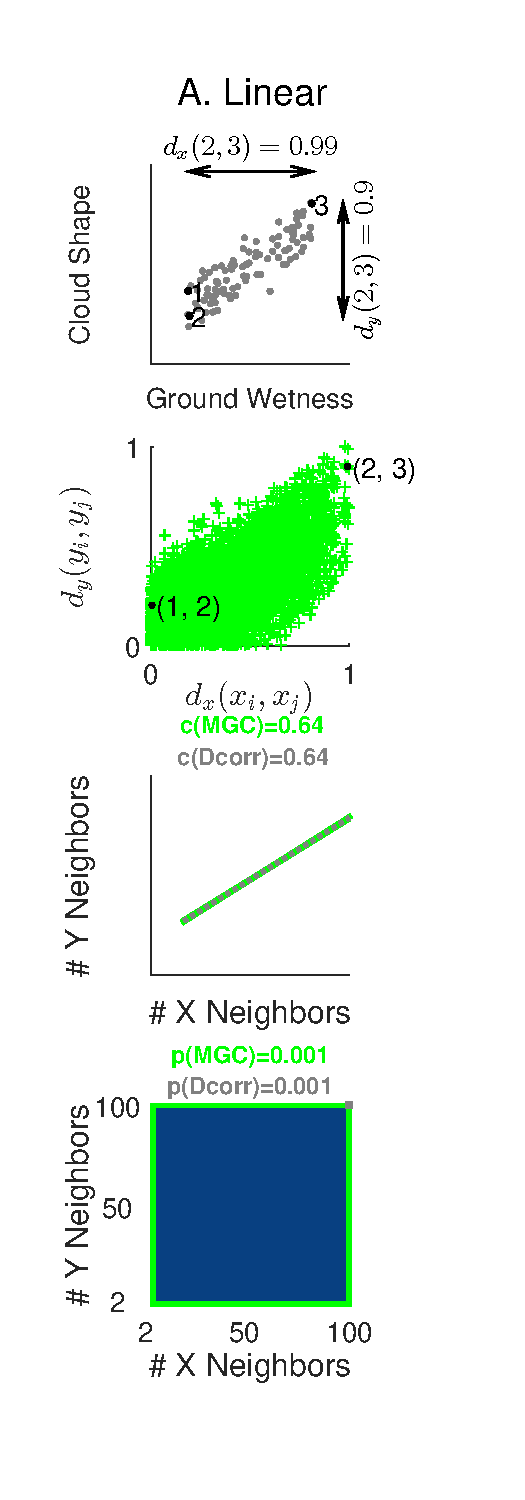
\includegraphics[width=1.0\textwidth]{../Figures/Fig1}
\caption{
Power of different methods on 20 different one-dimensional simulation settings, estimated on the basis of 10000 Monte-Carlo replicates.
Each panel shows empirical testing power on the absicca, and sample size on the ordinate.
LGC empirically achieves as high or higher power than the previous state of the art approaches for nearly all sample sizes on nearly all problems.}
\label{fig:1D}
\end{figure}


\subsection{High Dimensional Simulation Experiments}
\label{numer2}
In this subsection we consider the same $20$ distributions and the same testing procedures, but in an increasing dimension setting. The sample size is fixed at $n=100$, with increasing $d_{x}$ and no noise in this simulation; $d_{y}$ is either fixed at $1$ or increases together with $d_{x}$, depending on the particular distribution. The empirical testing powers based on $r=10000$ Monte-Carlo replicates at $\alpha=0.05$ is plotted in Figure~\ref{fig:nD} against the dimension $d_{x}$.

Similarly, we provide the performance profiles in the third and fourth panel of Figure~\ref{fig:pp} for the increasing dimension scenario: the third panel draws the performance profiles of all methods at a fixed dimension determined by a power threshold; and the fourth panel plots the area under curve of the performance profiles against the power threshold.

For the increasing dimension scenario, LGC significantly surpasses all other methods: for close to linear dependencies from type 1-5, LGC is as good as mcorr, whose power deteriorates much slower than the others; and for the remaining nonlinear dependencies, LGC is much better than all methods including mcorr, due to its capability to better handle non-linearity and high-dimensionality at the same time. The advantage is also reflected in the performance profiles of LGC in Figure~\ref{fig:pp}. %Note that a quarter of the distributions (e.g. sine period, square, diamond) cannot be detected by any method at dimension higher than $1$, since the testing powers quickly degrade to around $\alpha$.


\begin{figure}[htbp]
\subfloat[]{
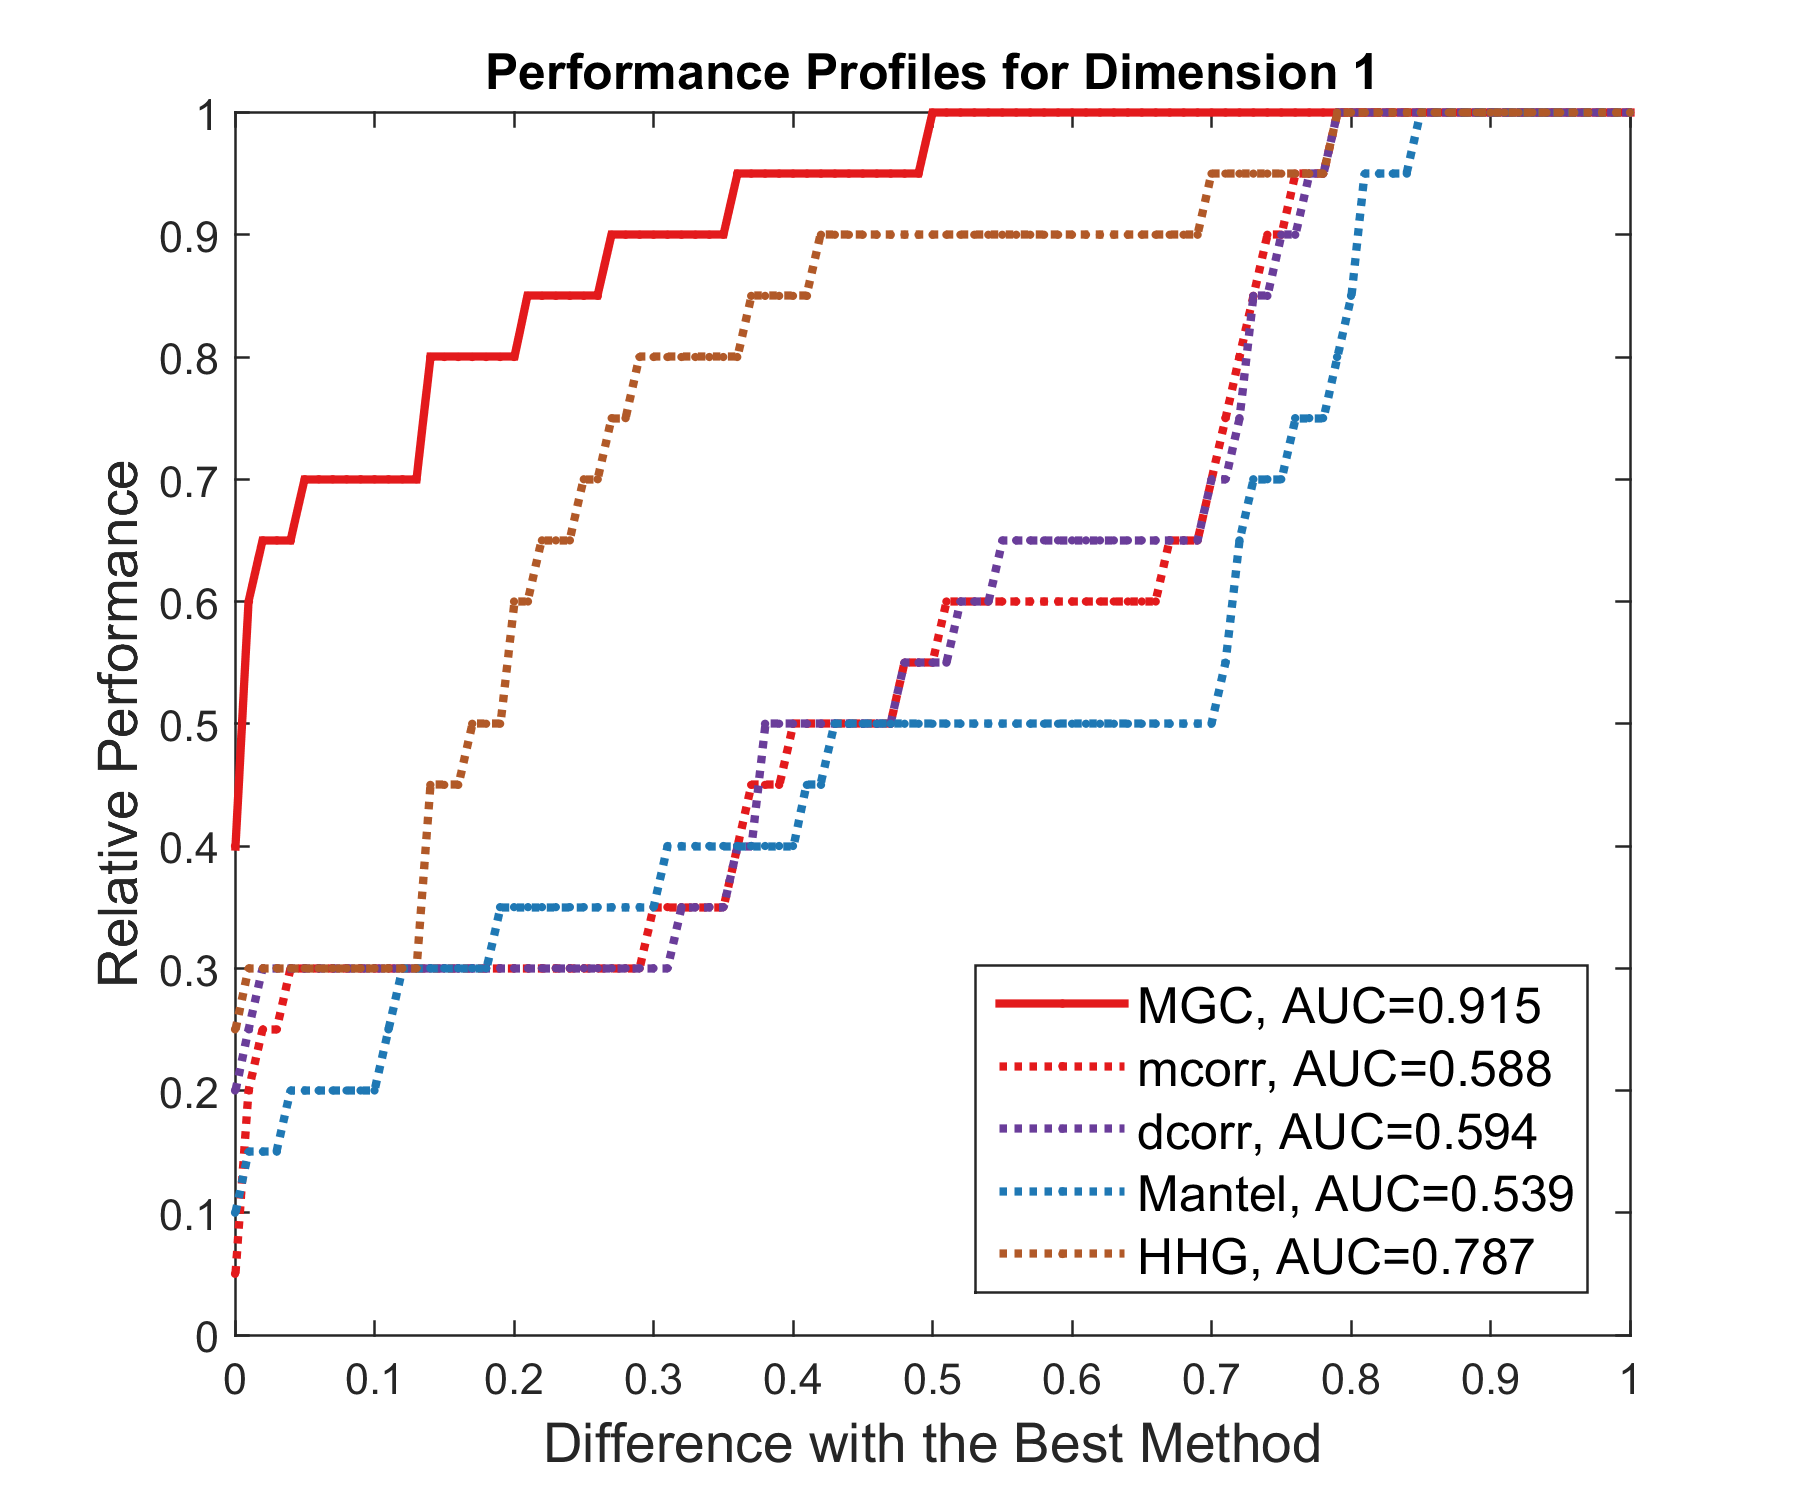
\includegraphics[width=0.5\textwidth]{../Figures/Fig3}
}
\hfil
\subfloat[]{
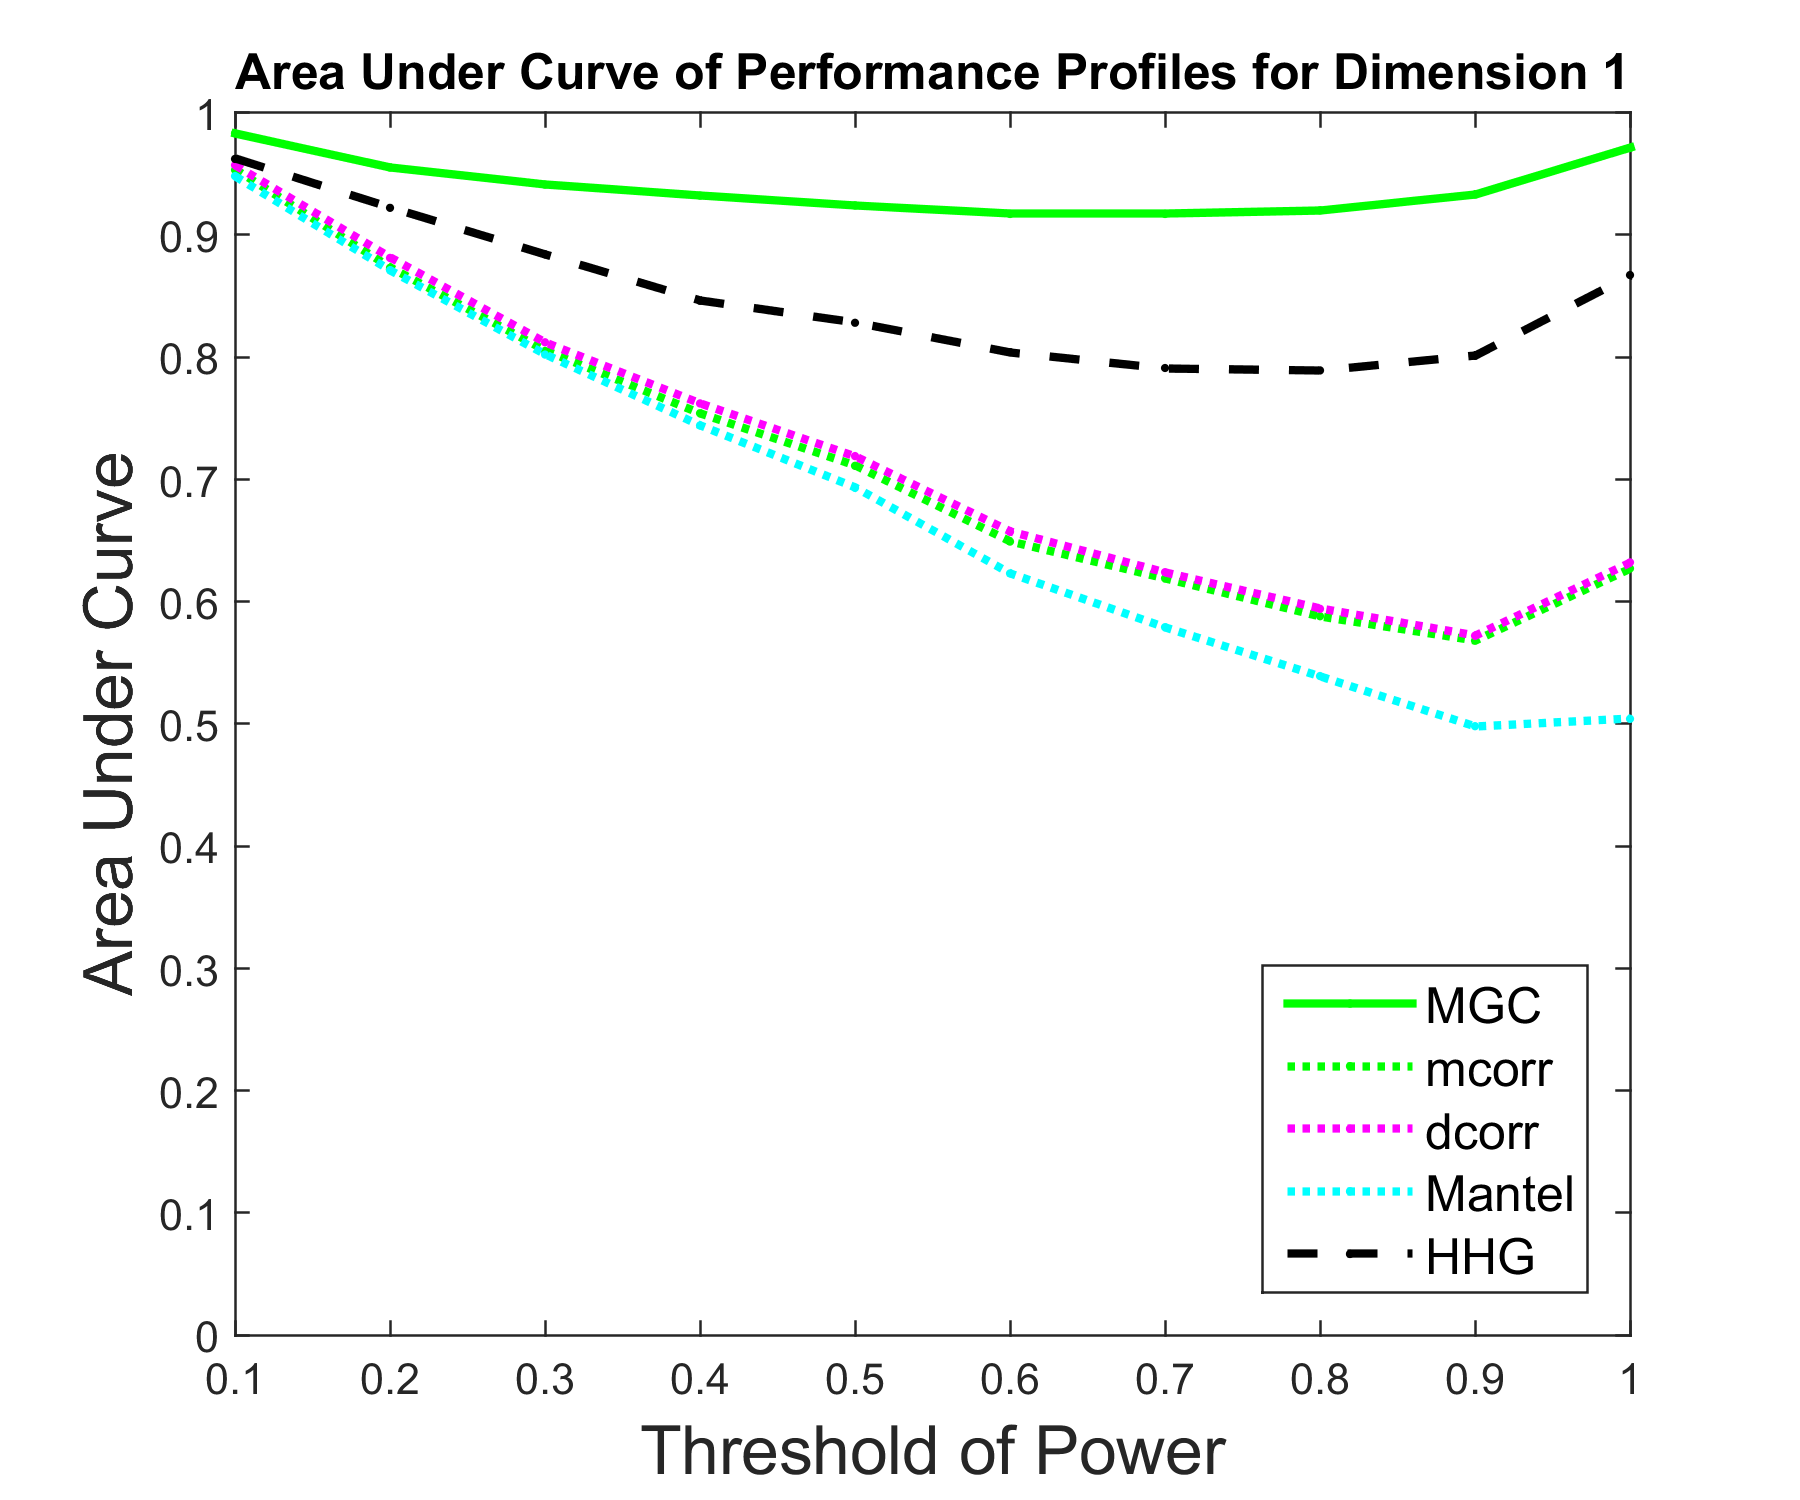
\includegraphics[width=0.5\textwidth]{../Figures/Fig4}
}
\hfil
\subfloat[]{
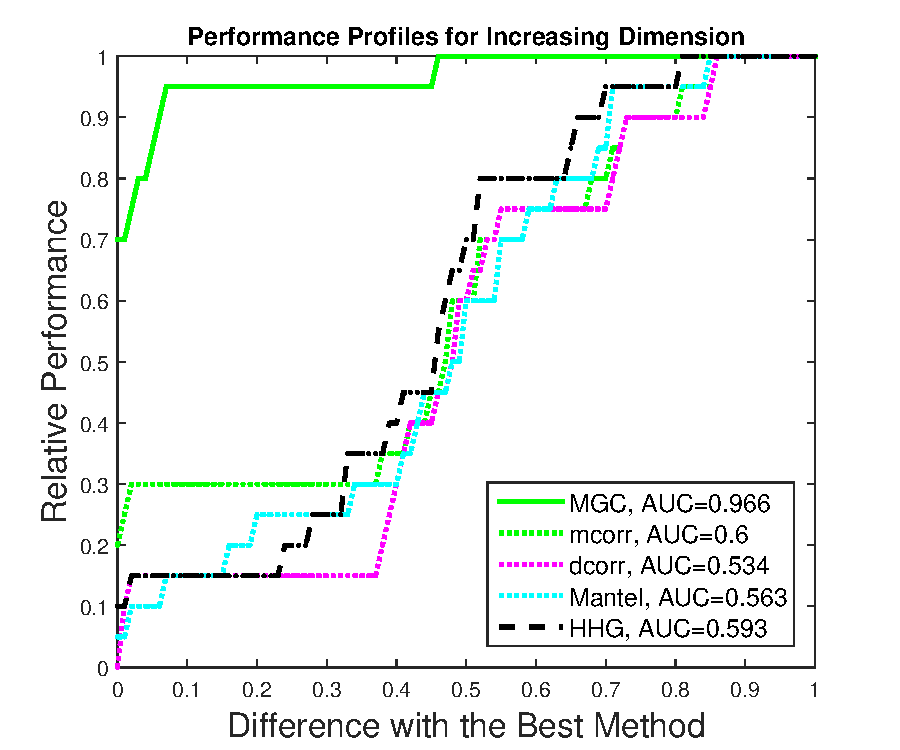
\includegraphics[width=0.5\textwidth]{../Figures/Fig7}
}
\hfil
\subfloat[]{
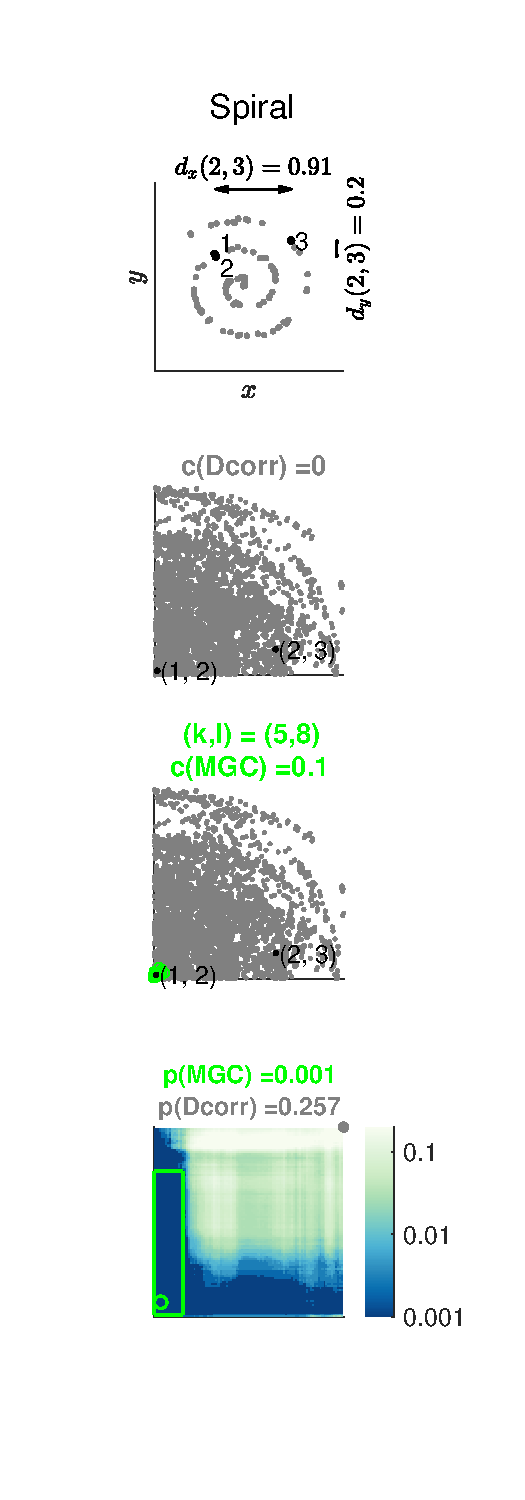
\includegraphics[width=0.5\textwidth]{../Figures/Fig8}
}
\caption{Quantitative comparisons of the power of the various algorithms across all simulations into a single number.  
(a) Performance profile plots comparing the different algorithms on all 1-dimensional problems at the first sample size $n$ of any testing power to exceed the power threshold 0.8. The legend provides the Area-Under-the-Curve (AUC) for each method; larger is better.
(b) AUC for each method sweeping over all different power thresholds.
(c) Same as (a) but for the high-dimensional simulations, at the last dimension of any testing power that is above the power threshold 0.5 YYY tried to fix the description again, clear now or not?YYY XXX the previous clause is not clear to me XXX.
(d) Same as (b) but for the high-dimensional simulations.
It is clear that our method outperforms the previous state of the art, regardless of function, sample size, and dimensionality.}
\label{fig:pp}
\end{figure}




\begin{figure}[htbp]
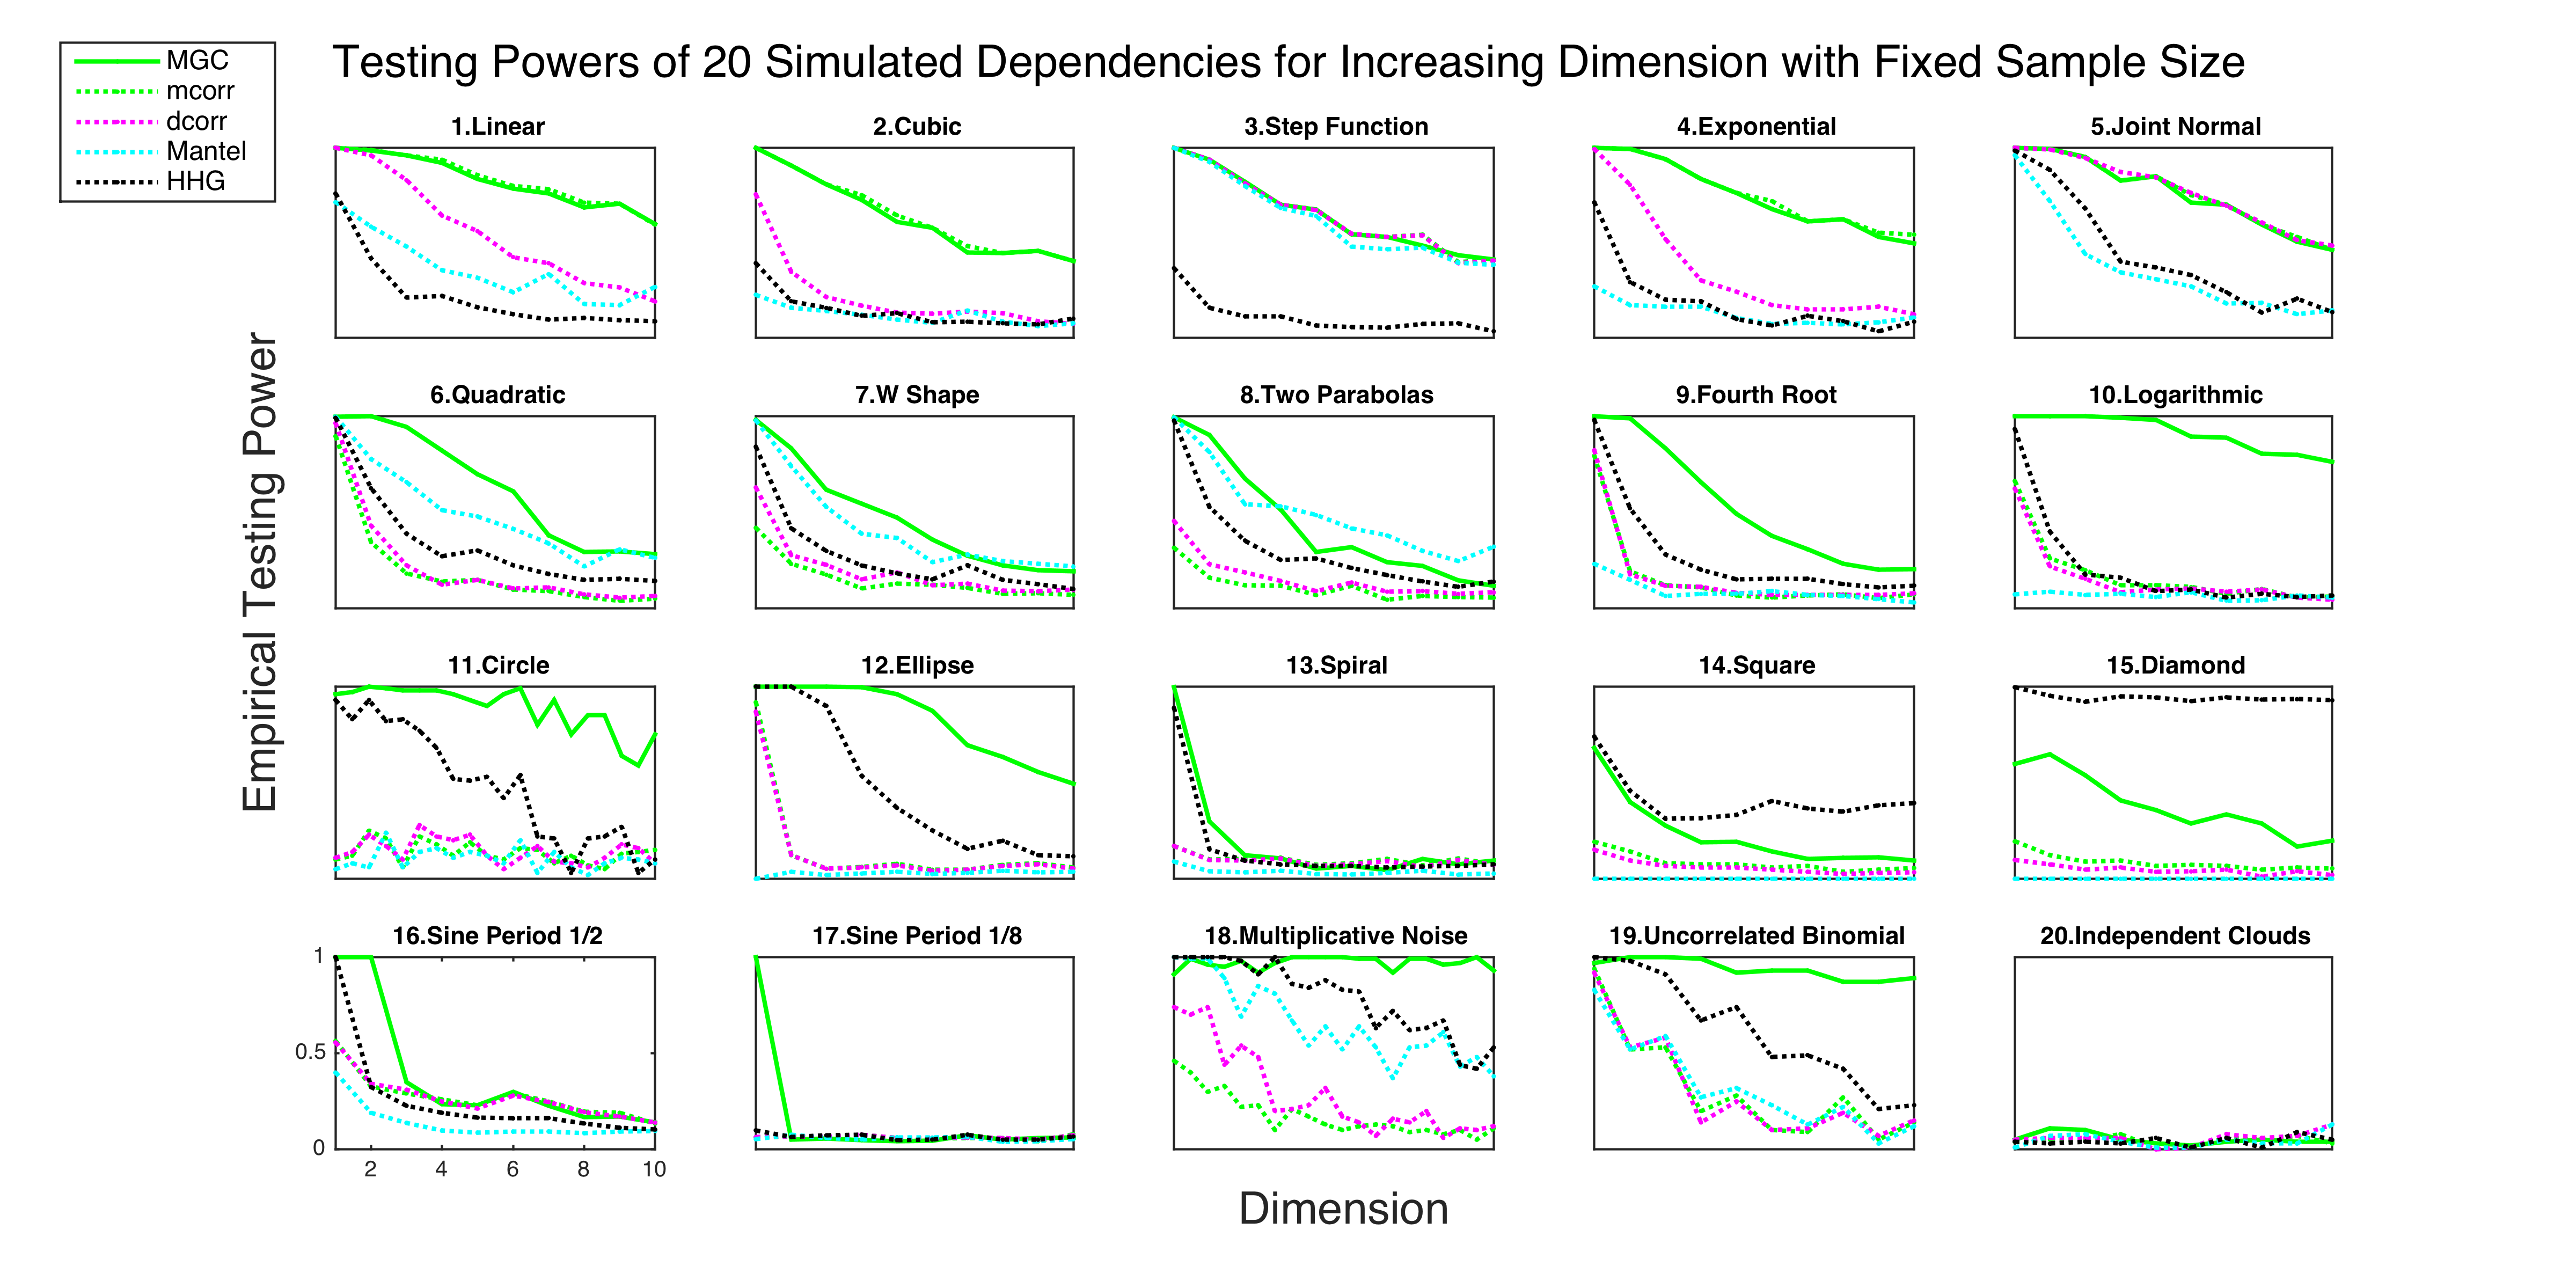
\includegraphics[width=1.0\textwidth]{../Figures/Fig5}
\caption{Power of different methods on 20 different simulation settings, for dimensionality ranging from 1 to 1000.  Details as in Figure~\ref{fig:1D}.
Again, our method empirically achieves as high or higher power than the previous state of the art approaches for nearly all sample sizes on nearly all problems and dimensions.
}
\label{fig:nD}
\end{figure}



\subsection{Discovery of Dependency Across Scales}


XXX add discussion about discovering dependency across scales. XXX
YYY below paragraph used to be in appendix; moved here after I notice you put the corresponding figures in this section YYY

In Figure~\ref{figSim2} we show how the powers of $g_{kl}$ change with respect to increasing neighborhood $k$ and $l$, for the low-dimension and high-dimension simulations. They are plotted at a fixed sample size and a fixed dimension by the same thresholds as the performance profiles figures. We can clearly see that for consecutive neighborhoods, the local testing powers are very close to each other, since the local tests are strongly correlated with each other. This implies that the optimal neighborhood choice of LGC can be reasonably estimated by bootstrap.

\begin{figure}[htbp]
\subfloat[]{
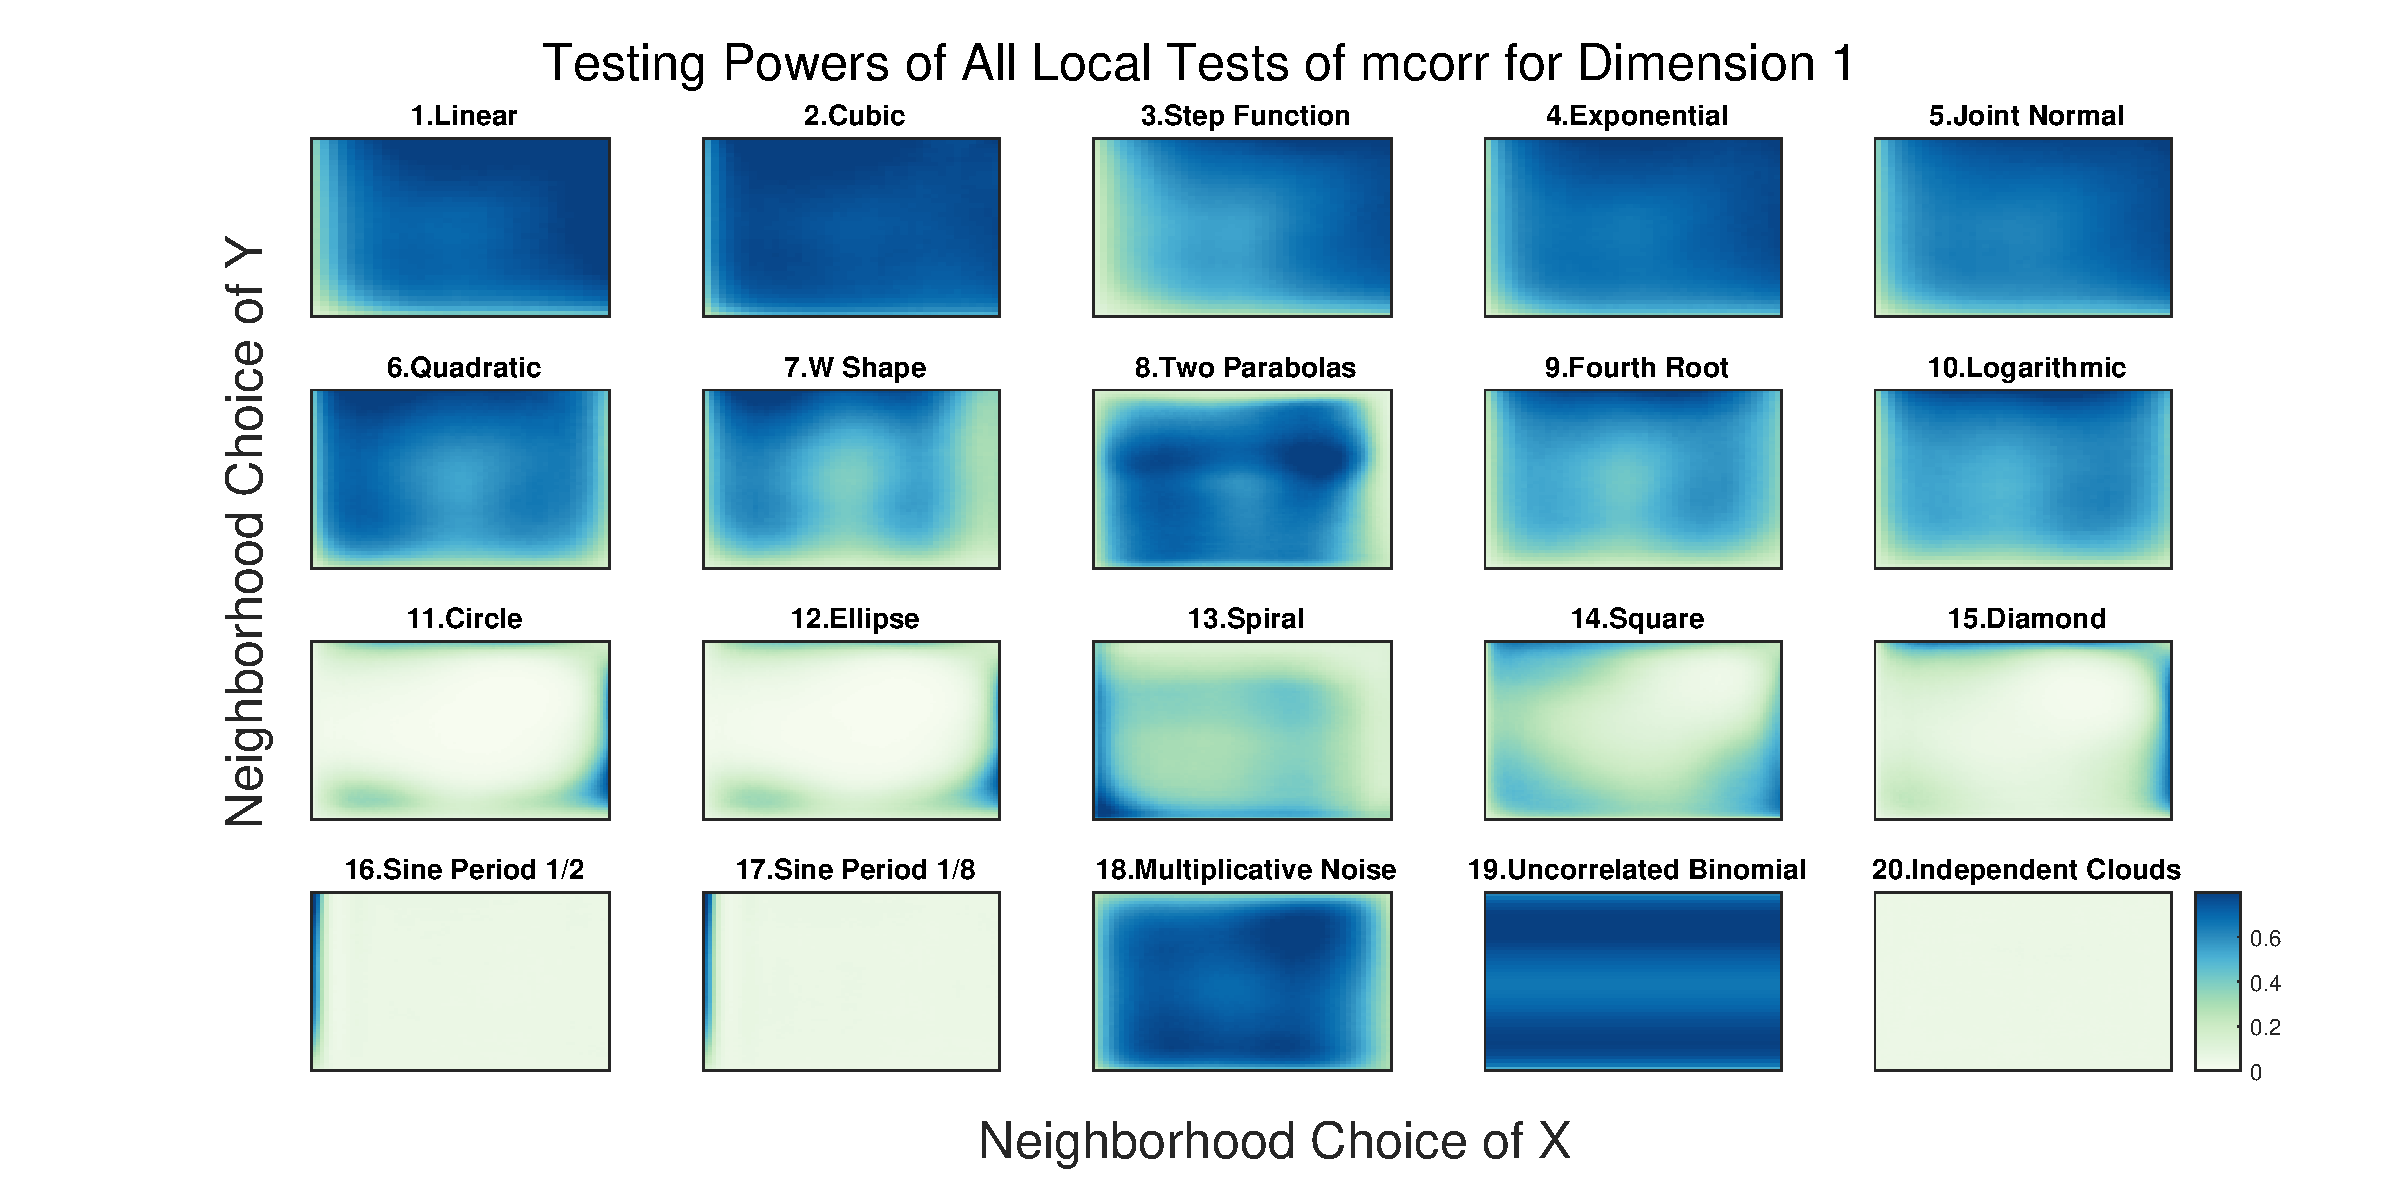
\includegraphics[width=1.0\textwidth]{../Figures/Fig2}
}
\hfil
\subfloat[]{
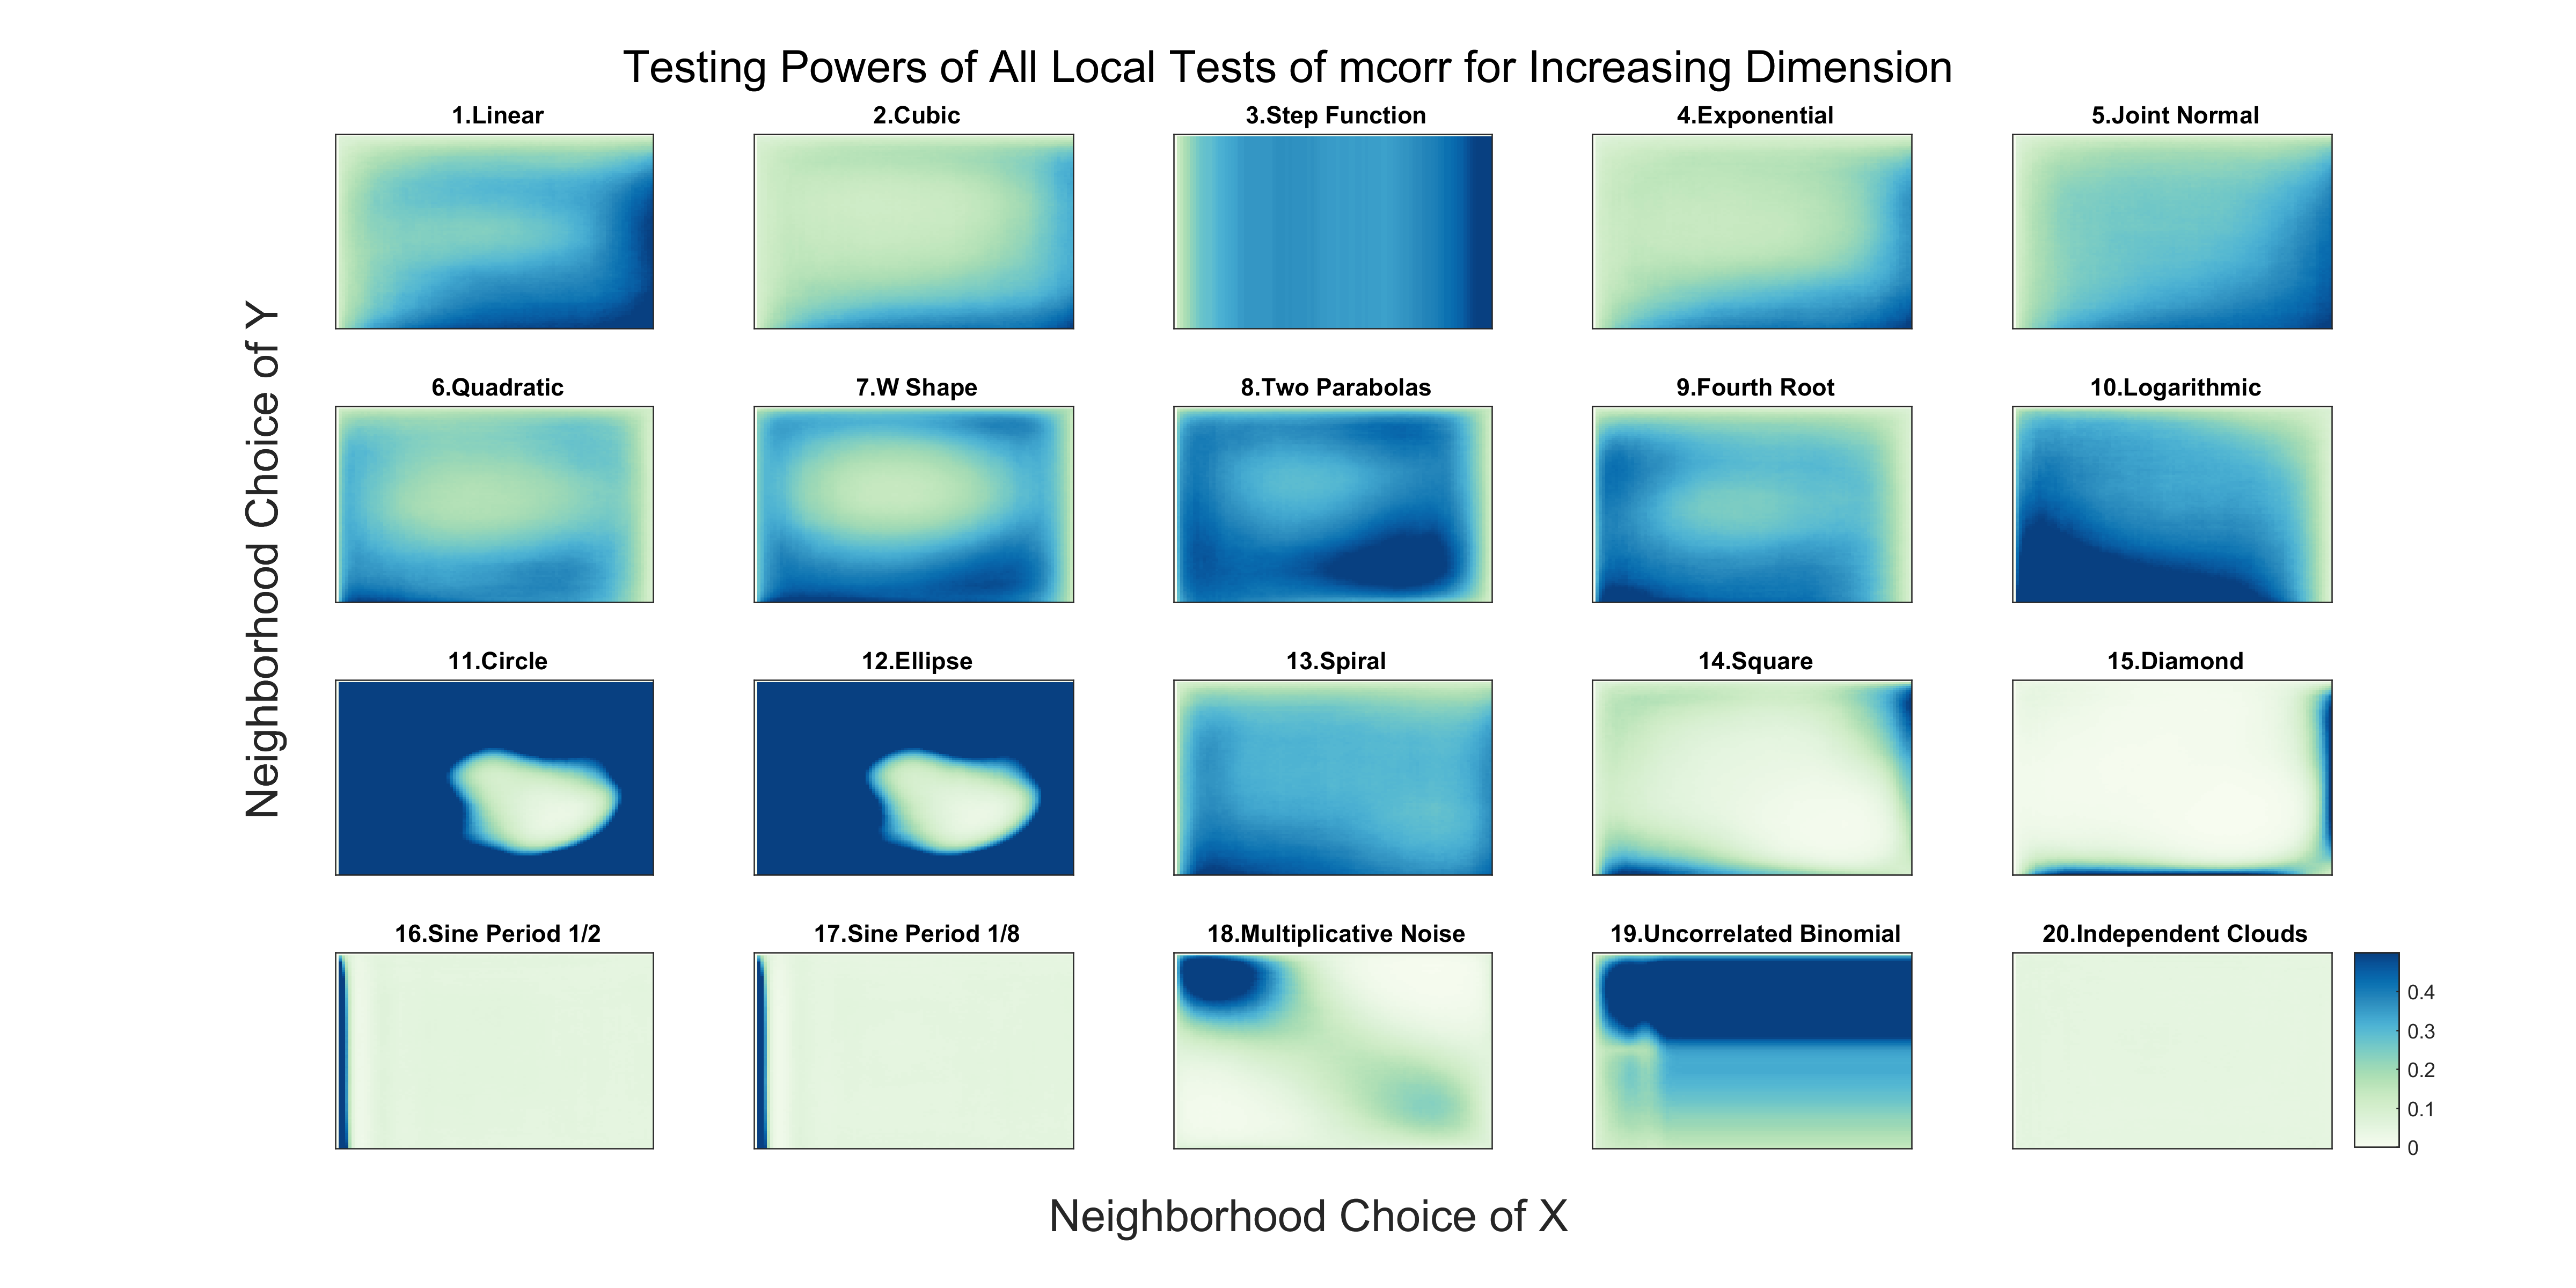
\includegraphics[width=1.0\textwidth]{../Figures/Fig6}
}
\caption{Testing Power Heat-map of Local Graph Correlation for Dimension 1 and Increasing Dimension.
% Understanding how dependence varies with the local scale of the dependence.  
For each of the 20 panels, the abscissa denotes the number of neighbors for $X$, and the ordinate denotes the number of neighbors for $Y$.  Each different simulation yields a different surface, highlighting the importance of understanding local scale in terms of understanding the data.}
\label{figSim2}
\end{figure}

\subsection{Real Data}
\label{numer3}
Here we apply LGC to test independence between brain features and personal characteristics from two different experiments, for which the data sets are relatively small in sample size due to the expensive data collection process. We report the p-values of all test statistics from the permutation test; and the optimal neighborhood size of LGC is estimated by bootstrap, based on the main algorithm in Section~\ref{main3} of the appendix.

The first experiment is to detect the relationship between the brain connectome and personality from \cite{AdelsteinEtAl2011}. The sample size is $n=42$, and each person has a $5$ dimensional personality data based on questionnaires and the five-factor personality model. Then the brain activity of each person is measured by fMRI for $197$ brain regions and $194$ time steps. Thus the brain connectome feature is high-dimensional while the personality data is low-dimensional. There seems to exist certain correlation between the brain activity and personality as experimentally shown in \cite{AdelsteinEtAl2011}, but whether the dependency can be detected from the raw data is the question here.

To apply our method, two distance measures are required for the two different data sources: for the personality data, the distance matrix is formed by the Euclidean distance directly; for the connectome data, we run a spectrum analysis for each region, bandpass and normalize it, then calculate the Kullback-Leibler divergence among regions and use the normalized Hellinger distance. Once the distance matrices are obtained, we apply the permutation test in Section~\ref{main3} for $r=10000$ random permutations, and show the p-values (the percentage that the test statistic between the permuted data is larger than the observed test statistic) of LGC, dcorr, mcorr, Mantel, and HHG in the first row of Table~\ref{table1}, with the smallest p-value highlighted in the table.

In this experiment, only LGC by mcorr yields significant p-value that is less than $0.05$, and the estimated optimal neighborhood choice is $k^{*}=9, l^{*}=4$ based on $10000$ bootstrap samples. No other method yields significant p-value, although HHG is quite close. We also show the p-value heat map of the local tests with respect to all possible neighborhoods in the first plot of Figure~\ref{figReal}, and we can clearly see a local structure in the data that yield significant p-values for adjacent neighborhoods.

Note that if we use LGC by dcorr rather than mcorr, the p-value is no longer significant: this implies a high-dimensional structure in the dependency, which is indeed the case for the connectome data. Also note that the distance measure (especially for the connectome data) may not be the most appropriate for detecting dependency, and it is possible that HHG and dcorr may yield better p-values under different metrics.

\begin{table*}[!t]
\footnotesize
\renewcommand{\arraystretch}{0.5}
\centering
{\begin{tabular}{|c||c|c|c|c|c|c|c|}
\hline
Testing Method & LGC by mcorr & LGC by dcorr & LGC by Mantel & mcorr & dcorr & Mantel & HHG \\
\hline
Connectome x Personality & $\textbf{0.0331}$ & $0.9489$  & $0.1321$ & $0.3244$ & $0.6534$ & $0.9830$  & $0.0582$ \\
\hline
Left Brain vs Disorder  & $0.0235$ & $0.0270$ & $\textbf{0.0146}$ & $0.0789$ & $0.0712$ & $0.0383$ & $0.0388$ \\
\hline
Right Brain vs Disorder & $\textbf{0.0126}$ & $0.0148$  & $0.0306$ & $0.1139$ & $0.1055$  & $0.0766$ & $0.0861$\\
\hline
\end{tabular}
\caption{The Empirical P-Value of Permutation Test}
\label{table1}
}
\end{table*}


\begin{figure}[htbp]
\centering
\subfloat[]{
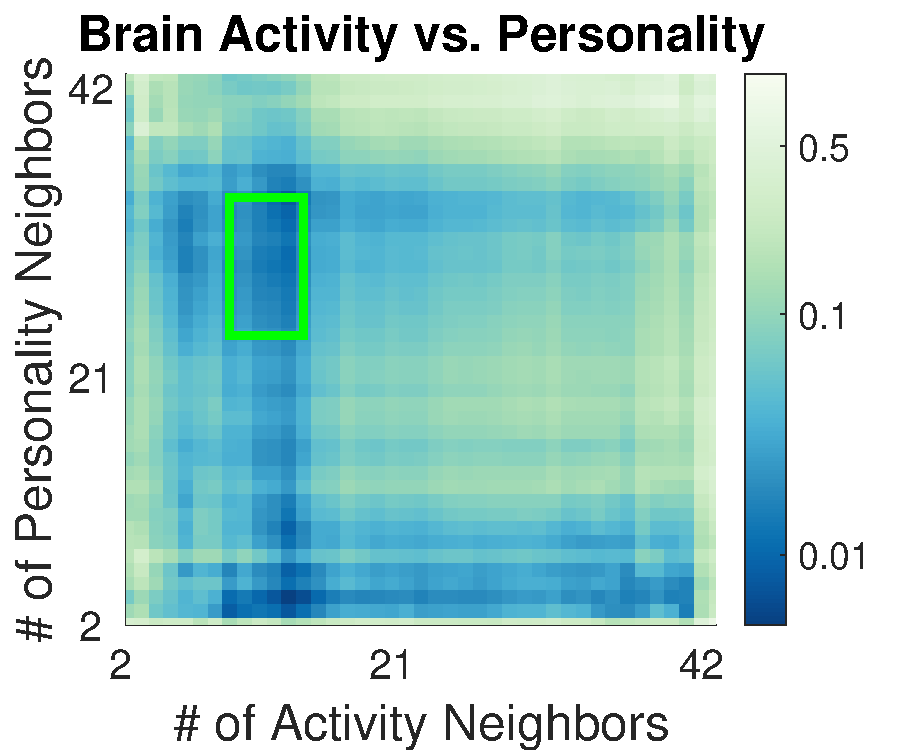
\includegraphics[width=0.48\textwidth]{../Figures/FigReal1}
}
\hfil
\centering
\subfloat[]{
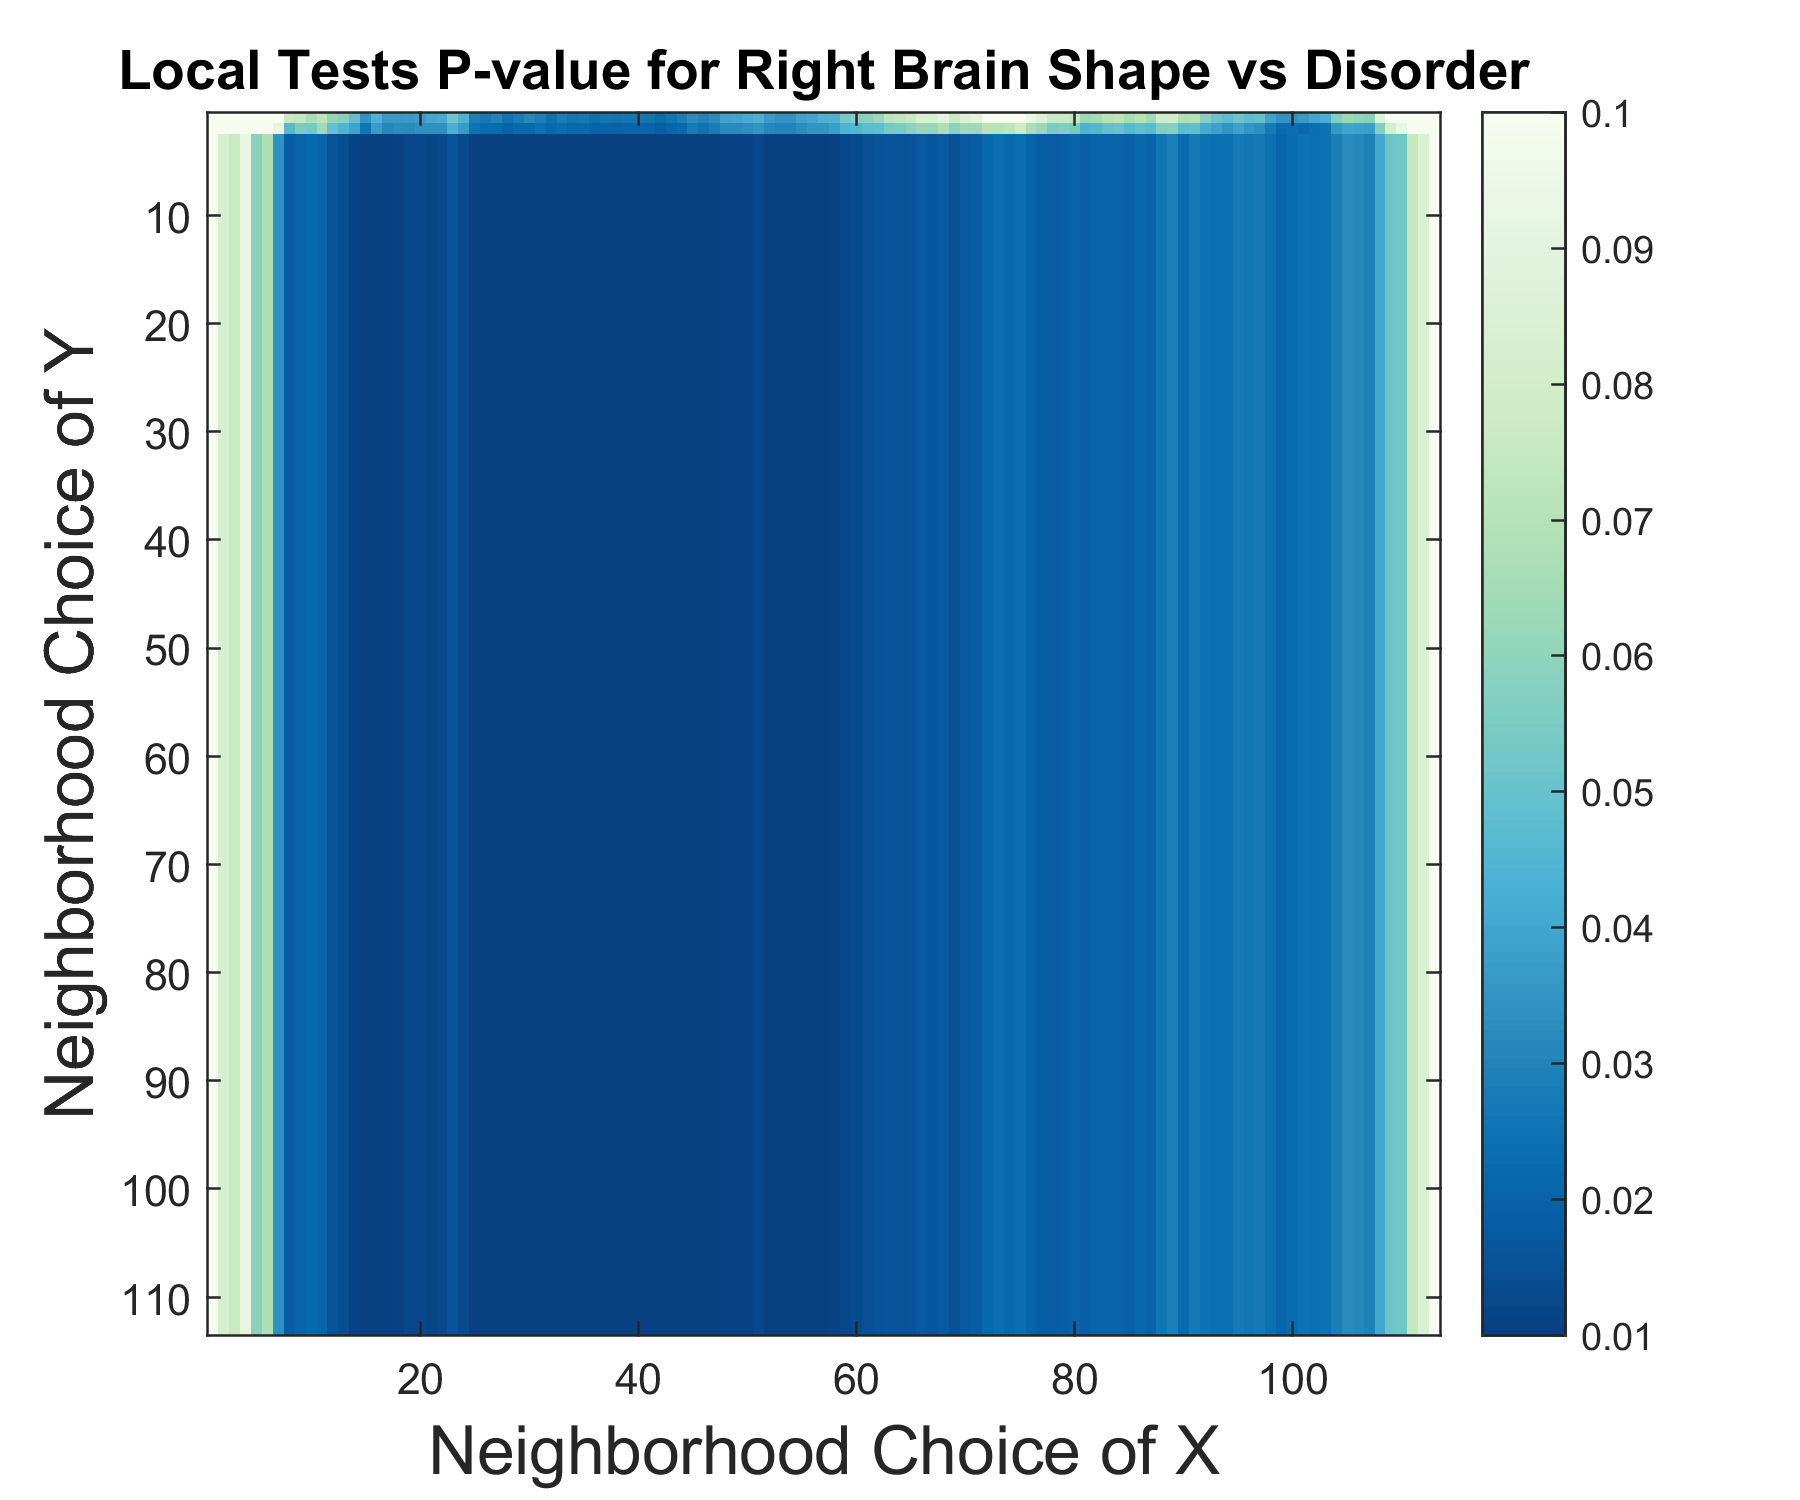
\includegraphics[width=0.48\textwidth]{../Figures/FigReal2}
}
\hfil
\centering
\subfloat[]{
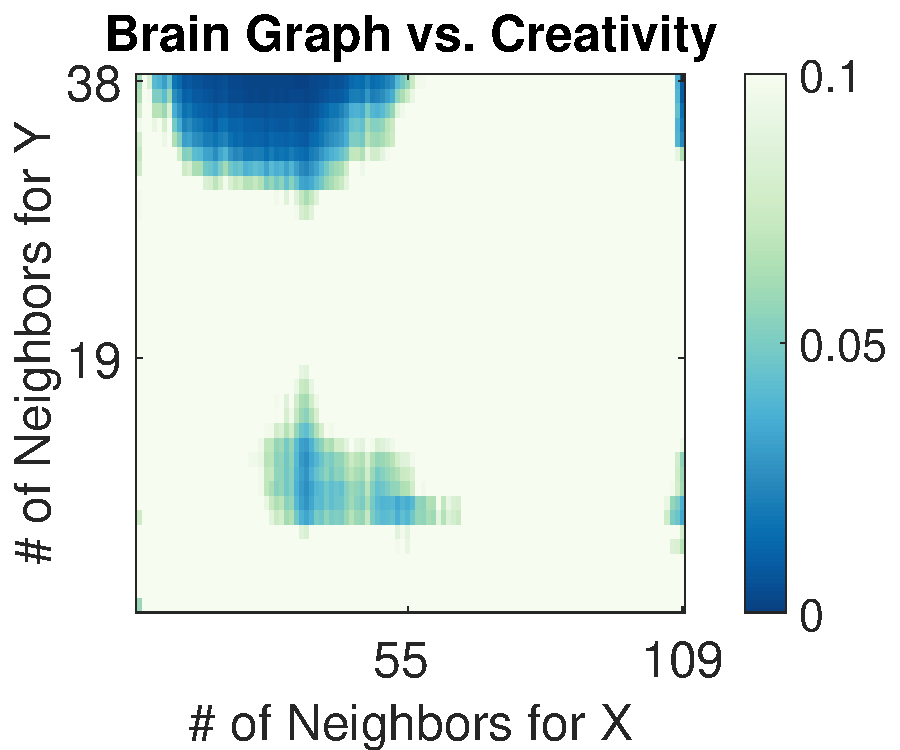
\includegraphics[width=0.48\textwidth]{../Figures/FigReal3}
}
\caption{P-Value Heatmap of Local Graph Correlation with respect to Different Neighborhood Choice.  In the real data, for the personality vs. graph dependency, global structure is inadequate to reveal any dependence between the two modalities.  For the shape vs. status,  global distances are sufficient.  XXX we still need the example where we fail to detect dependence when it does not exist.  you have everything you need for that? XXX}
\label{figReal}
\end{figure}

Next we carry out the same testing procedure on another experiment regarding brain hippocampus shape and major depressive disorder. There are $n=114$ subjects, and the brain images of each person are obtained by high resolution MRI scans on the hippocampus; and we also have available a categorical vector containing the disorder information, including clinically depressed subject, high-risk subject, and non-affected subject. There has been evidences that relate major depressive disorder to the hippocampus shape in \cite{ParkEtAl2011} and \cite{PosenerEtAl2003}, and we would like to test the significance of such relationship in the data. 

The brain data is transformed into two dissimilarity matrices representing the left and right hippocampus data based on landmark matching (see \cite{ParkEtAl2011} for more details on data processing). The disorder information vector is transformed into its Euclidean distance with all off-diagonal entries added by $1$, so that only the diagonals are zero, and subjects of the same disorder status have smaller distance than subjects of different disorder status.

We consider two hypothesis tests: testing dependency between the left brain and major depressive disorder, and testing dependency between the right brain and major depressive disorder. The resulting p-values are reported in the second and third rows of Table~\ref{table1}.

For testing between the left brain and the disorder, all methods yield significant p-values with LGC by Mantel being the most significant; and there exists more than one optimal neighborhood for LGC based on $10000$ bootstrap samples, with the heat map provided in the second plot of Figure~\ref{figReal}. For testing between the right brain and the disorder, only local tests yield significant p-values, although all global tests are not too far away from significant; again there exists more than one optimal neighborhood for LGC, with the heat map provided in the third plot of Figure~\ref{figReal}. 

%We can observe from the heat map of LGC that there is a clear threshold in the local structure most neighborhood choices after certain threshold yields significant p-values, and LGC with mcorr performs similarly as LGC with dcorr. They imply that the dependency between the brain data and the disease data is probably cross-region, close to linear and low-dimensional. Furthermore, the left brain seems to be more correlated with the disease than the right brain, as testing between $LML$ and $D$ yields smaller p-values than testing between $LMR$ and $D$.

The results indicate a nonlinear low-dimensional dependency between the brain and major depressive disorder. Note that if we test dependency between the left and right brain, all p-values become $0$, indicating a strong linear dependency between the left and right brain.

\section{Discussion}
\label{conclu}

\paragraph{Summary}

In short, we propose local graph correlation to test independence between data sets, which has been shown to be perform well for testing independence on data of small sample size, high-dimensionality, linearity or non-linearity. It not only enjoys theoretical guarantee such as being consistent in testing independence, but also exhibits superior numerical performances in a comprehensive simulation setting and real data experiments, comparing to other popular methods.


\paragraph{Next Steps}

one-sample, two-sample, group testing, anova, regressing out other covariates (local partial correlation), screening, metric spaces.

different test statistics: there are many possible ways to generate the null distribution, including permutation, but also t-test (as in the mcorr paper and the asymptotic distribution derived from Gretton et al 2009), wilcoxon signed rank test, etc..


scaling up via FlashX?

\section*{Acknowledgment}
\addcontentsline{toc}{section}{Acknowledgment}
This work was partially supported by 
% 
National Security Science and Engineering Faculty Fellowship (NSSEFF), 
% 
Johns Hopkins University Human Language Technology Center of Excellence (JHU HLT COE), 
% 
Defense Advanced Research Projects Agency's (DARPA) SIMPLEX program through SPAWAR contract N66001-15-C-4041, 
% 
and the XDATA program of the Defense Advanced Research Projects Agency (DARPA) administered through Air Force Research Laboratory contract FA8750-12-2-0303.



\appendix
\setcounter{figure}{0}
\renewcommand\thefigure{\arabic{figure}} 

\section{Functions}
\label{appen:a}

Here we list the distributions of the $20$ dependencies used in the simulation sections, most of which are based on the numerical settings in \cite{SzekelyRizzoBakirov2007, SimonTibshirani2012, SimonTibshirani2012, GorfineHellerHeller2012}. 

For the purpose of the increasing dimension scenario, we denote $w$ as a size $1 \times d_{x}$ vector with $w_{i}=\frac{1}{i}$. So $w\mb{x}$ is a dimension $1$ random variable that is a decaying weighted summation of $\mb{x}$, which equals $\mb{x}$ when $d_{x}=1$. In the following, $\mb{u}, \mb{v}$ are auxiliary random variables, $c$ is a scalar constant to control the noise level, and $\epsilon$ denotes the standard normal distribution for white noise unless mentioned otherwise. The resulting pair of random variables $(\mb{x},\mb{y})$ are used to generate sample data for testing dependency.

1. Linear: $\mb{x} \sim uniform(-1,1)^{d_{x}}$, $\mb{y}=w\mb{x}+c\epsilon$. 

2. Cubic: $\mb{x} \sim uniform(-1,1)^{d_{x}}$, $\mb{y}=128(w\mb{x}-\frac{1}{3})^3+48(w\mb{x}-\frac{1}{3})^2-12(w\mb{x}-\frac{1}{3})+80c\epsilon$.

3. Step function: $\mb{x} \sim uniform(-1,1)^{d_{x}}$, $\mb{y}=I(w\mb{x}>\hat{E}(w\mb{x}))+c\epsilon$, where $\hat{E}(w\mb{x})$ denotes the sample mean of $w\mb{x}$ and $I$ is the indicator function. 

4. Exponential: $\mb{x} \sim uniform(0,3)^{d_{x}}$, $\mb{y}=exp(w\mb{x})+10c\epsilon$.

5. Joint normal: Set $d_{x}=d_{y}$. Denote $\rho=\frac{1}{2d_{x}}$, $I_{d_{x}}$ as the identity matrix of size $d_{x} \times d_{x}$, $J_{d_{x}}$ as the matrix of ones of size $d_{x} \times d_{x}$, and $\Sigma = \begin{bmatrix} I_{d_{x}}&\rho J_{d_{x}}\\ \rho J_{d_{x}}&I_{d_{x}} \end{bmatrix}$. Then let $(\mb{x},\mb{u}) \sim normal(0, \Sigma)$ and $\mb{y}=\mb{u}+0.5c\epsilon$.

6. Quadratic: $\mb{x} \sim uniform(-1,1)^{d_{x}}$, $\mb{y}=(w\mb{x})^2+0.5c\epsilon$.

7. W Shape: $\mb{x} \sim uniform(-1,1)^{d_{x}}$, $\mb{u} \sim uniform(-1,1)^{d_{x}}$, $\mb{y}=4( ( (w\mb{x})^2 - \frac{1}{2} )^2 + w\mb{u}/500 )+0.5c\epsilon$.

8. Two Parabolas: $\mb{x} \sim uniform(-1,1)^{d_{x}}$, $\epsilon \sim uniform(0,1)$, $\mb{u} \sim Bernoulli(0.5)$, $\mb{y}=( (w\mb{x})^2  + 2c\epsilon) \cdot (\mb{u}-\frac{1}{2})$.

9. Fourth Root: $\mb{x} \sim uniform(-1,1)^{d_{x}}$, $\mb{y}=|w\mb{x}|^\frac{1}{4}+\frac{c}{4}\epsilon$.

10. Logarithmic: $\mb{x} \sim normal(0, 1)^{d_{x}}$, $\mb{y}=log(\mb{x}^2)+3c\epsilon$.

11. Circle: $\mb{x} \sim uniform(0,1)^{d_{x}}$, $\mb{u} \sim Bernoulli(0.5)$, $\mb{y}=((2\mb{u}-1) \cdot |1-(2\frac{w\mb{x}}{\max(w\mb{x})}-1)^2|^{\frac{1}{2}}+1)/2+0.1c\epsilon$.

12. Ellipse: Let $\mb{u} \sim uniform(-1,1)^{d_{x}}$, $\epsilon_{1} \sim normal(0,1)$, $\epsilon_{2} \sim normal(0,1)$. Then $\mb{x}=5w\sin(\pi \mb{u})+\frac{\epsilon_{1}}{8}$, $\mb{y}=w\cos(\pi \mb{u})+\frac{\epsilon_{2}}{3}$. 

13. Spiral: $\mb{u} \sim uniform(0,20)^{d_{x}}$, $\mb{x}=w\mb{u}w\sin(\mb{u})$,$\mb{x}=w\mb{u}w\cos(\mb{u})+0.4c\epsilon$. 

14. Square: Let $\mb{u} \sim uniform(-1,1)^{d_{x}}$, $\mb{v} \sim uniform(-1,1)^{d_{x}}$, $\theta=-\frac{\pi}{8}$. Then $\mb{x}=w\mb{u} \cos(\theta) + w\mb{v} \sin(\theta), \mb{y}=-w\mb{u} \sin(\theta) + w\mb{v} \cos(\theta)$. 

15. Diamond: Let $\mb{u} \sim uniform(-1,1)^{d_{x}}$, $\mb{v} \sim uniform(-1,1)^{d_{x}}$, $\theta=-\frac{\pi}{4}$. Then $\mb{x}=w\mb{u} \cos(\theta) + w\mb{v} \sin(\theta), \mb{y}=-w\mb{u} \sin(\theta) + w\mb{v} \cos(\theta)$. 

16. Sine Period 1/2: $\mb{x} \sim uniform(-1,1)^{d_{x}}$, $\mb{y}=sin(4\pi \frac{w\mb{x}}{\max(w\mb{x})})+c\epsilon$.

17. Sine Period 1/8: $\mb{x} \sim uniform(-1,1)^{d_{x}}$, $\mb{y}=sin(16\pi \frac{w\mb{x}}{\max(w\mb{x})})+0.5c\epsilon$.    

18. Multiplicative Noise: $\mb{x} \sim normal(0, 1)^{d_{x}}$, $\mb{u} \sim normal(0, 1)$, $\mb{y}=\mb{x} \cdot \mb{u}+0.5c\epsilon$.

19. Uncorrelated Binomial: $\mb{x} \sim Bernoulli(0.5)^{d_{x}}$, $\mb{u} \sim Bernoulli(0.5)$, $\mb{y}=w\mb{x} \cdot (2\mb{u}-1)+0.6c\epsilon$.

20. Independent Clouds: Let $\mb{u} \sim normal(0,1)^{d_{x}}$, $\mb{v} \sim normal(0,1)^{d_{y}}$, $\epsilon_{1} \sim Bernoulli(0.5)$, $\epsilon_{2} \sim Bernoulli(0.5)$. Then we set $d_{x}=d_{y}$, and take $\mb{x}=w\mb{u}/3+\epsilon_{1}, \mb{y}=w\mb{v}/3+\epsilon_{2}$.

For each distribution, $\mb{x}$ and $\mb{y}$ are clearly dependent (except type 20); and we can also generate independent data based on the same marginal distributions for the testing purpos. 

Our low-dimensional simulation is based on $d_{x}=d_{y}=1$ and $c=1$, with a visualization of all dependencies given in Figure~\ref{fig0}. Note that the constant before $c$ is tuned for each dependency type such that the testing power neither increases too fast or too slow, otherwise certain dependency in the absence of noise is very easy to be detected: say for type 1 linear, the testing powers of all methods converge to $1$ at very small $n$, such that we cannot meaningfully compare the methods.

The high-dimensional simulation is based on $c=0$ and increasing $d_{x}$, as the testing task is much more difficult for higher dimensions such that we no longer need additional noise to better compare different methods. Note that we can replace the fixed decaying vector $w$ by random decay, which still yield similar plots.

\begin{figure}[htbp]
\subfloat[]{
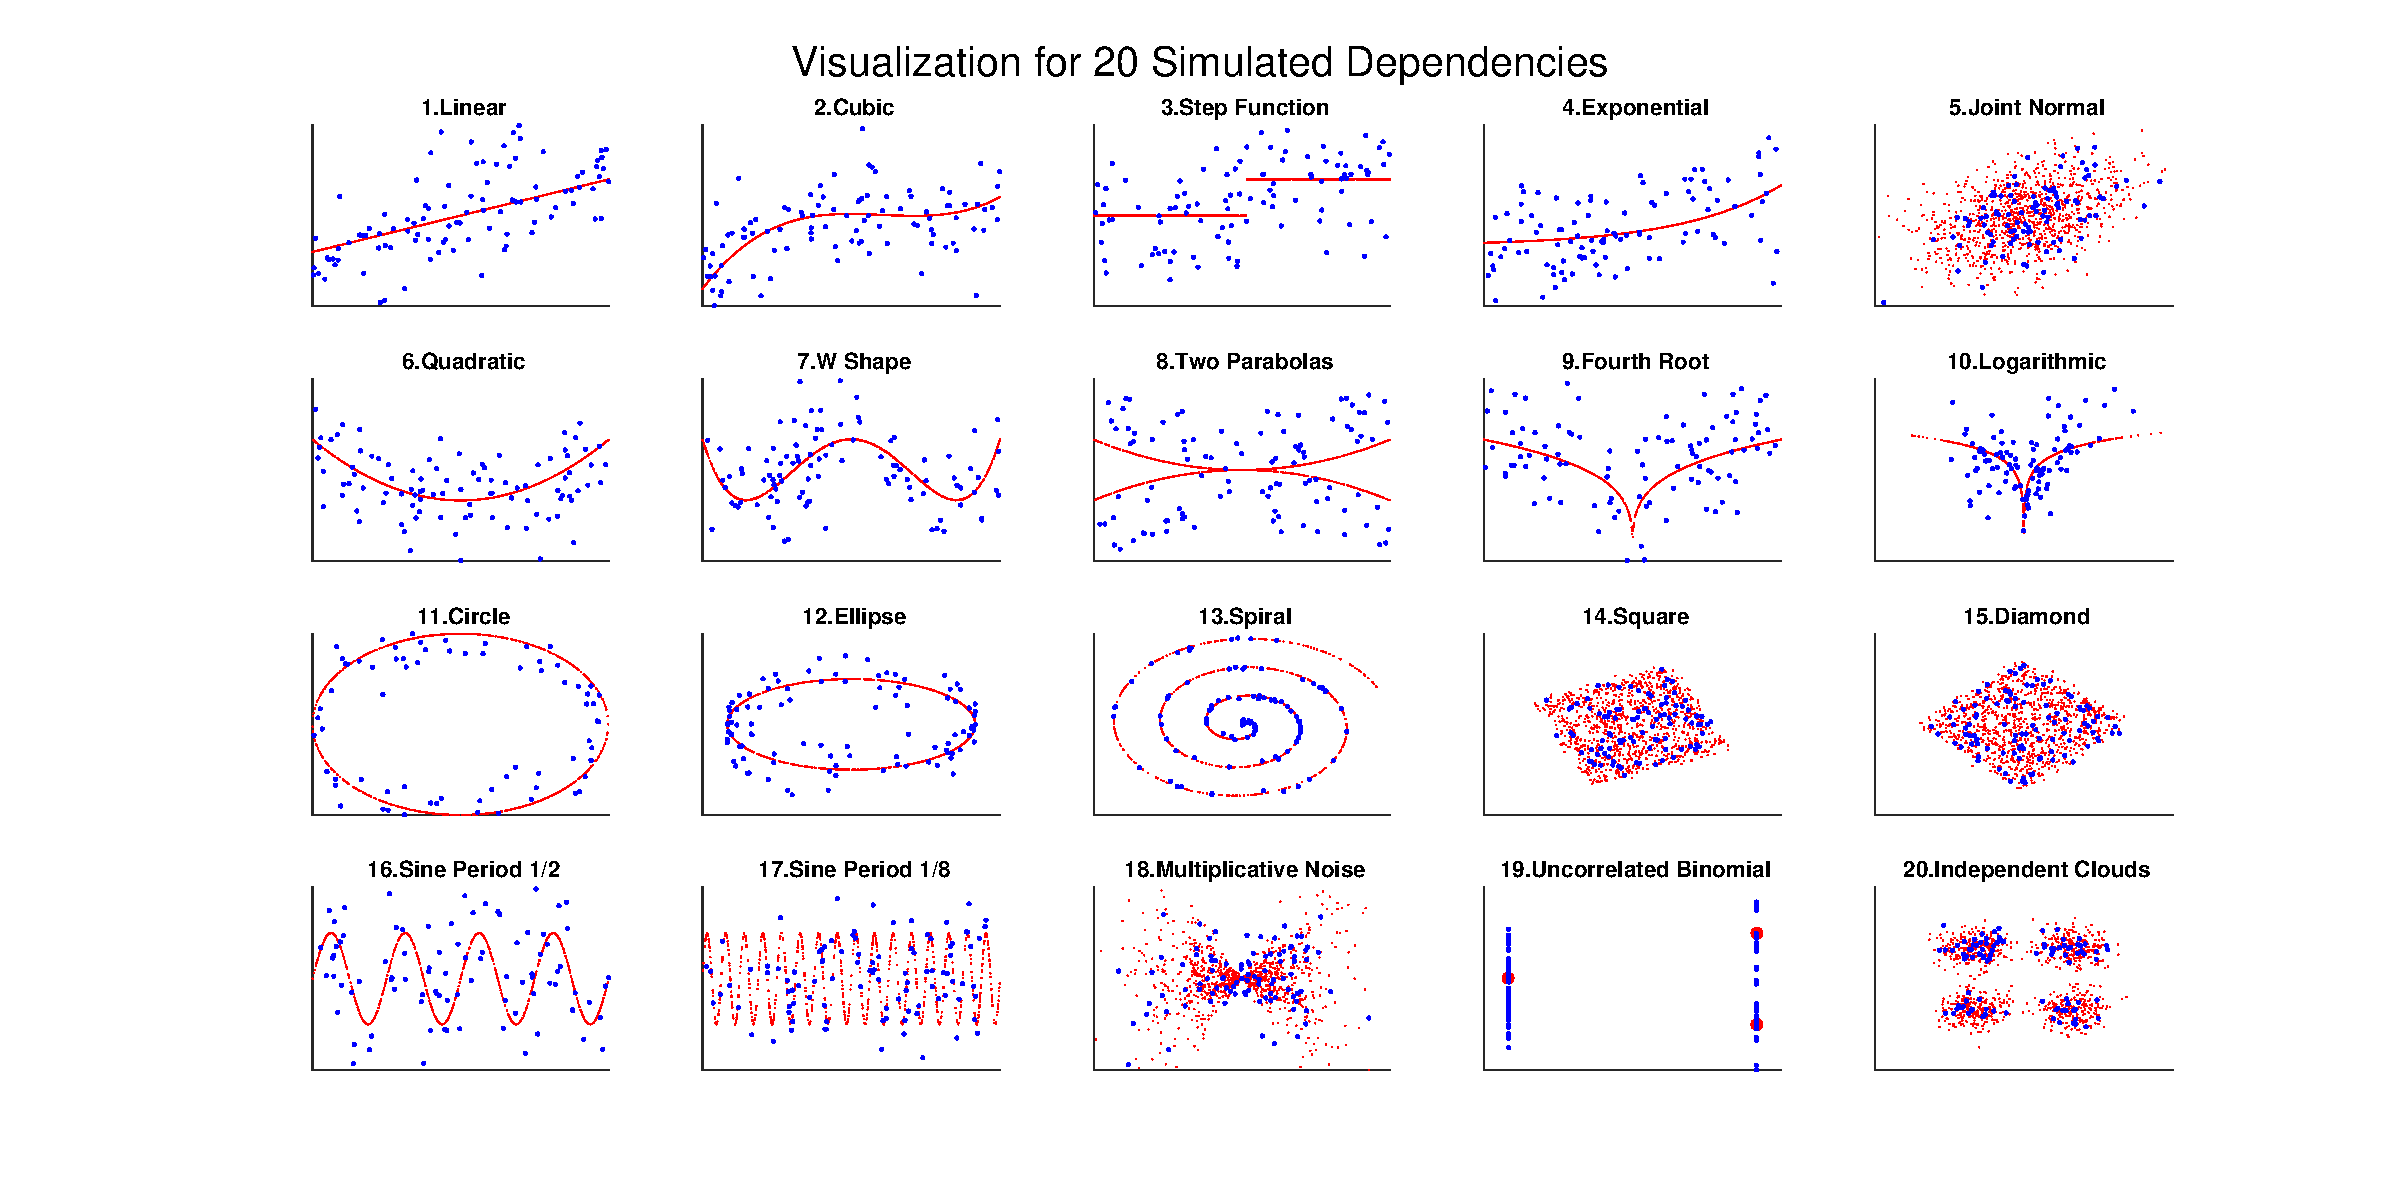
\includegraphics[width=1.0\textwidth]{../Figures/Fig0}
}
\caption{Visualization of 20 dependencies at dimension $1$. The blue points are generated with noise (c=1) for $n=100$ to show the actual sample data in testing, and the red points are generated with no noise (c=0) for $n=1000$ to highlight each underlying dependency.}
\label{fig0}
\end{figure}

\section{Supplementary Figures}

In Figure~\ref{fig:D2} and Figure~\ref{fig:pp2} we add the testing powers and performance profiles of LGC by dcorr and LGC by Mantel, for the same low-dimensional and high-dimensional scenarios in the main paper. Overall, LGC by dcorr and LGC by Mantel also improve over the respective global test statistics. Specifically, for the dimension 1 scenario, LGC by Mantel is overall slightly better than LGC by dcorr/mcorr due to its significant advantage for type 11-13; and for the increasing dimension scenario, LGC by Mantel/dcorr is similar to but slightly inferior to LGC by mcorr, due to the advantage of mcorr against high dimensional dependencies.

\begin{figure}[htbp]
\subfloat[]{
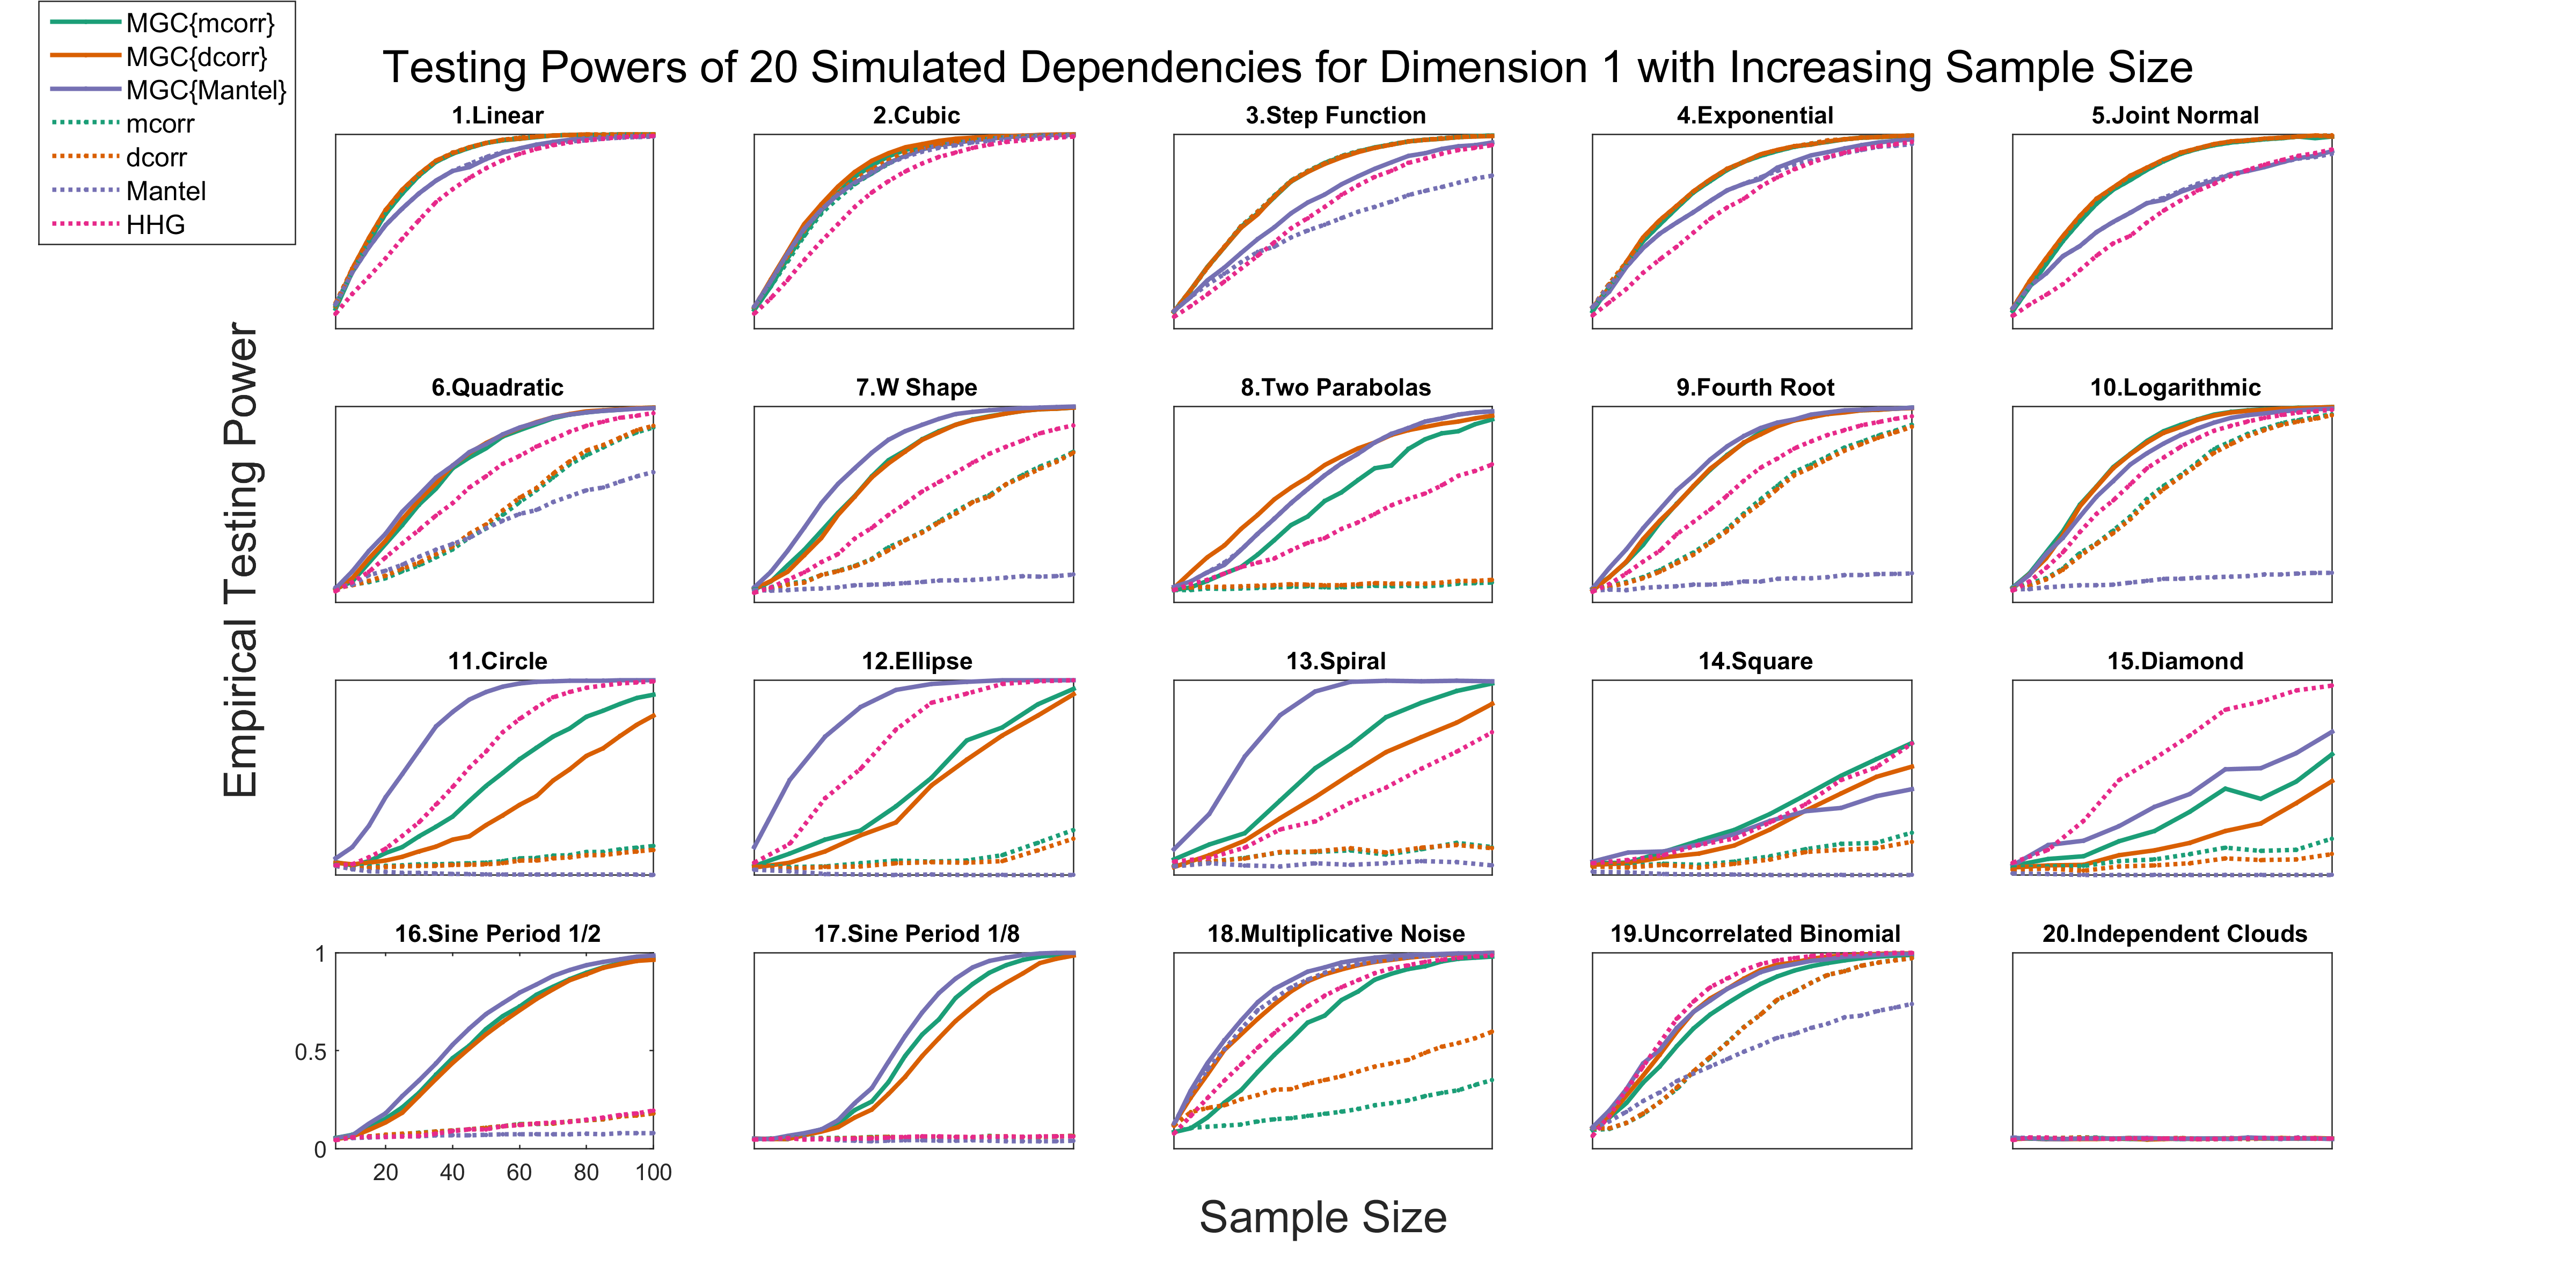
\includegraphics[width=1.0\textwidth]{../Figures/Fig1b}
}
\hfil
\subfloat[]{
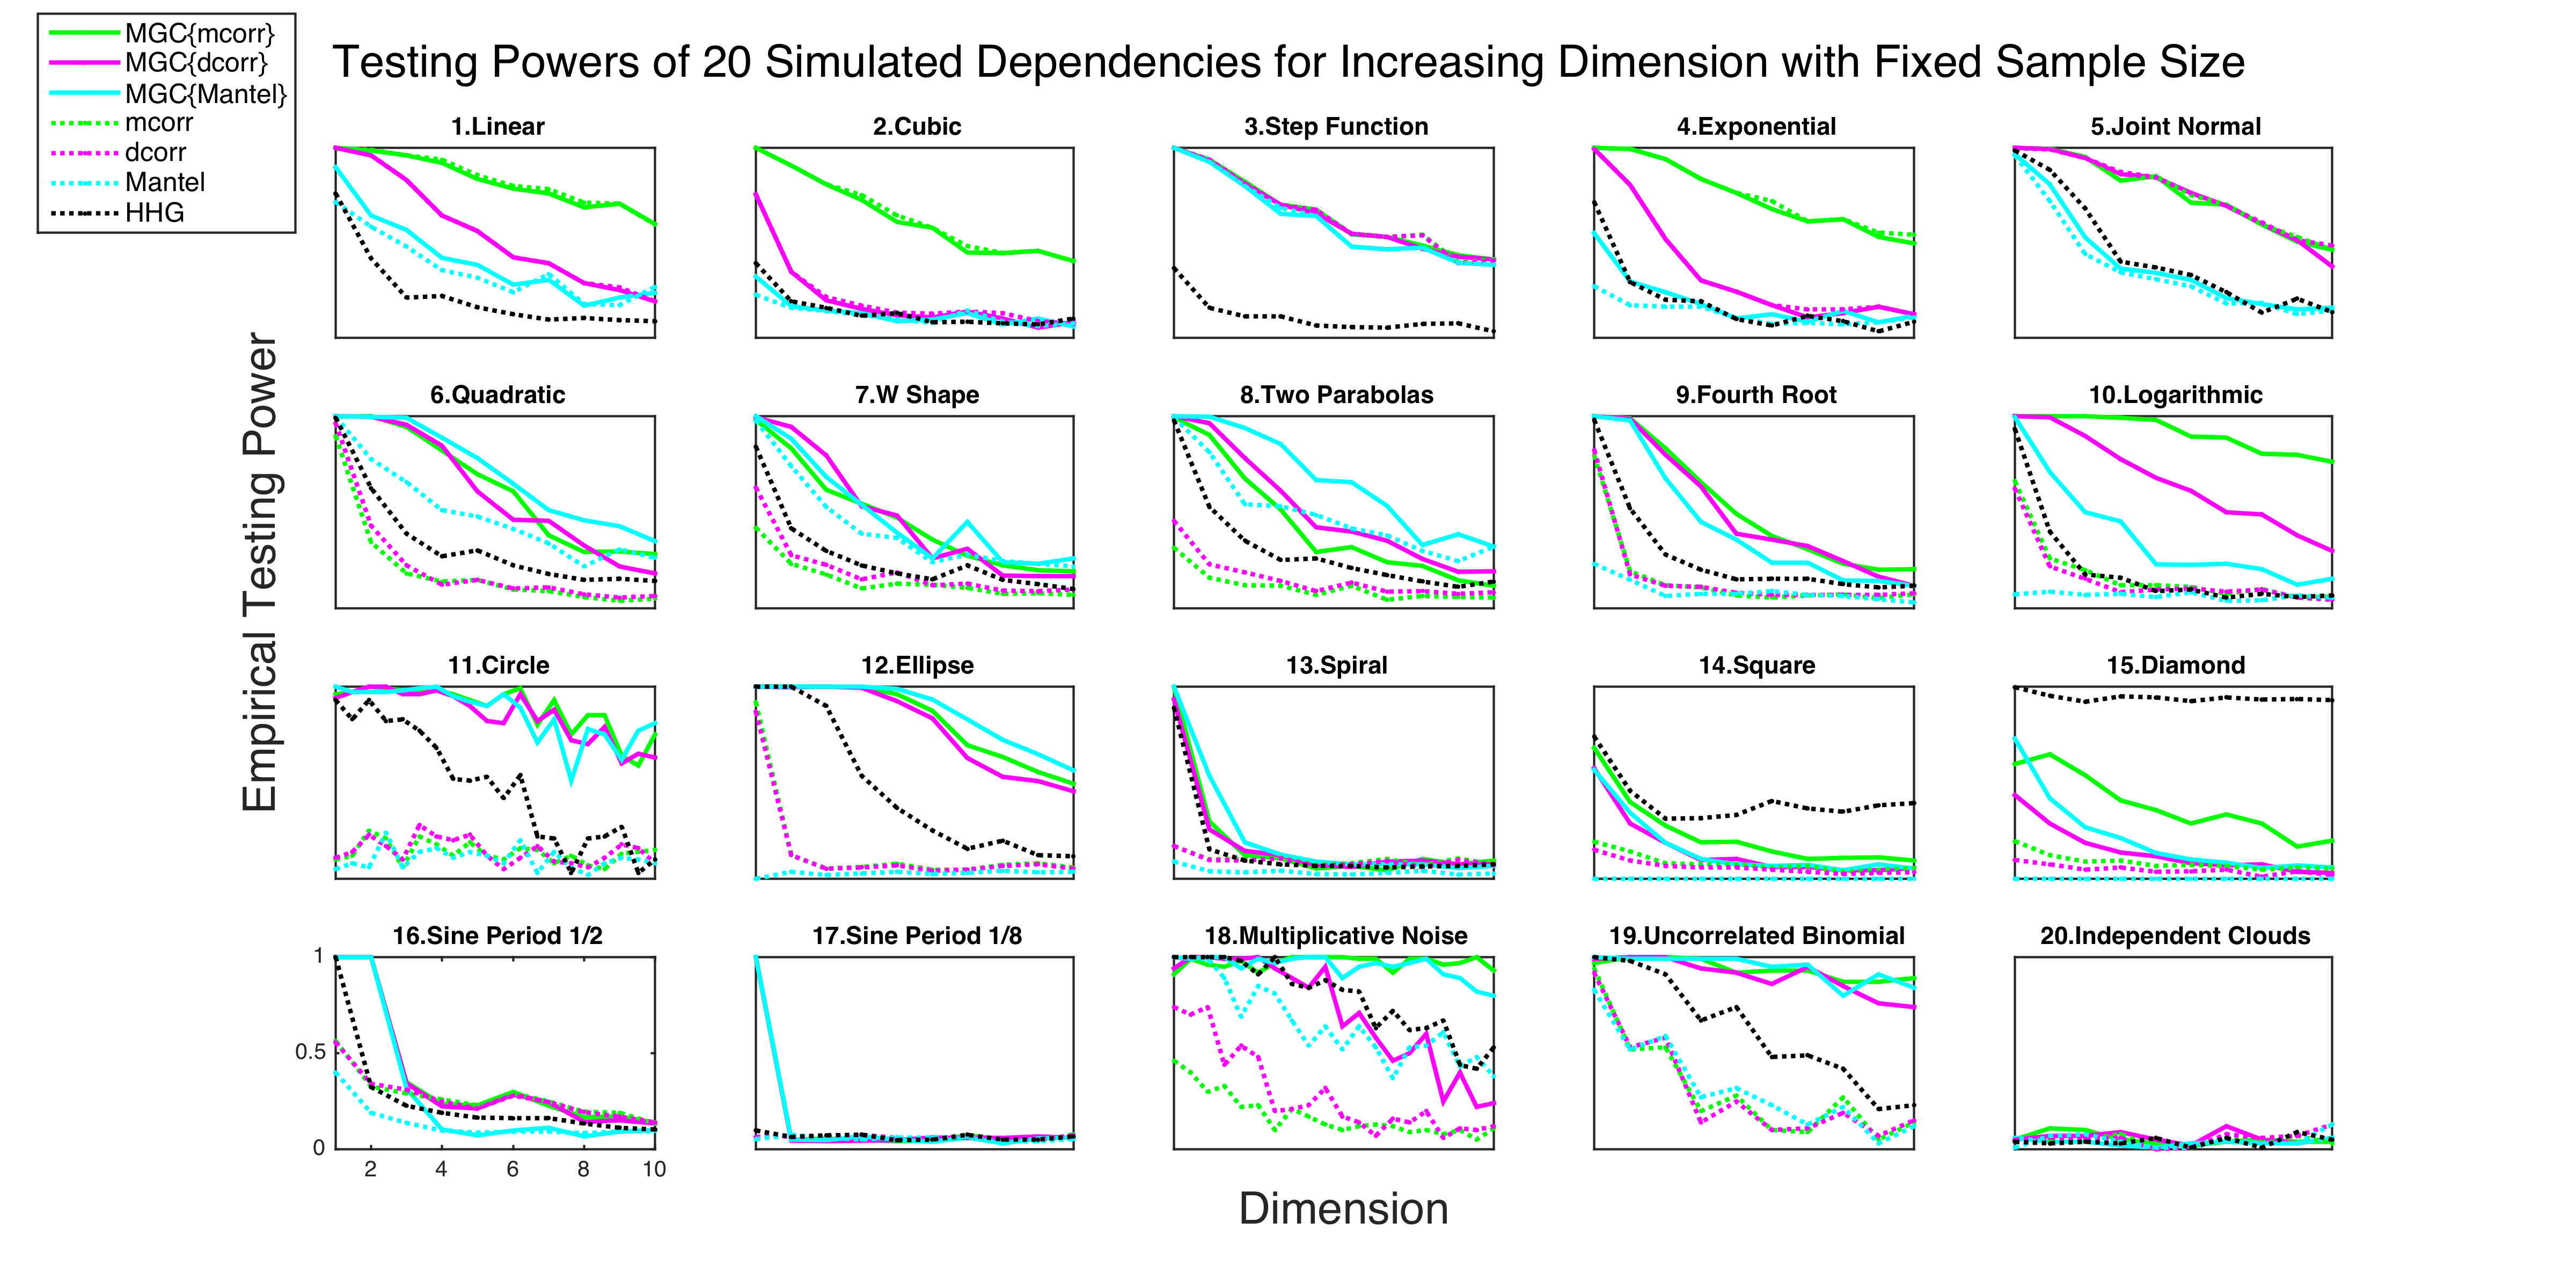
\includegraphics[width=1.0\textwidth]{../Figures/Fig5b}
}
\caption{Same Figures as Figure~\ref{fig:1D} and Figure\~ref{fig:nD}, adding in LGC by dcorr and LGC by Mantel}
\label{fig:D2}
\end{figure}

\begin{figure}[htbp]
\subfloat[]{
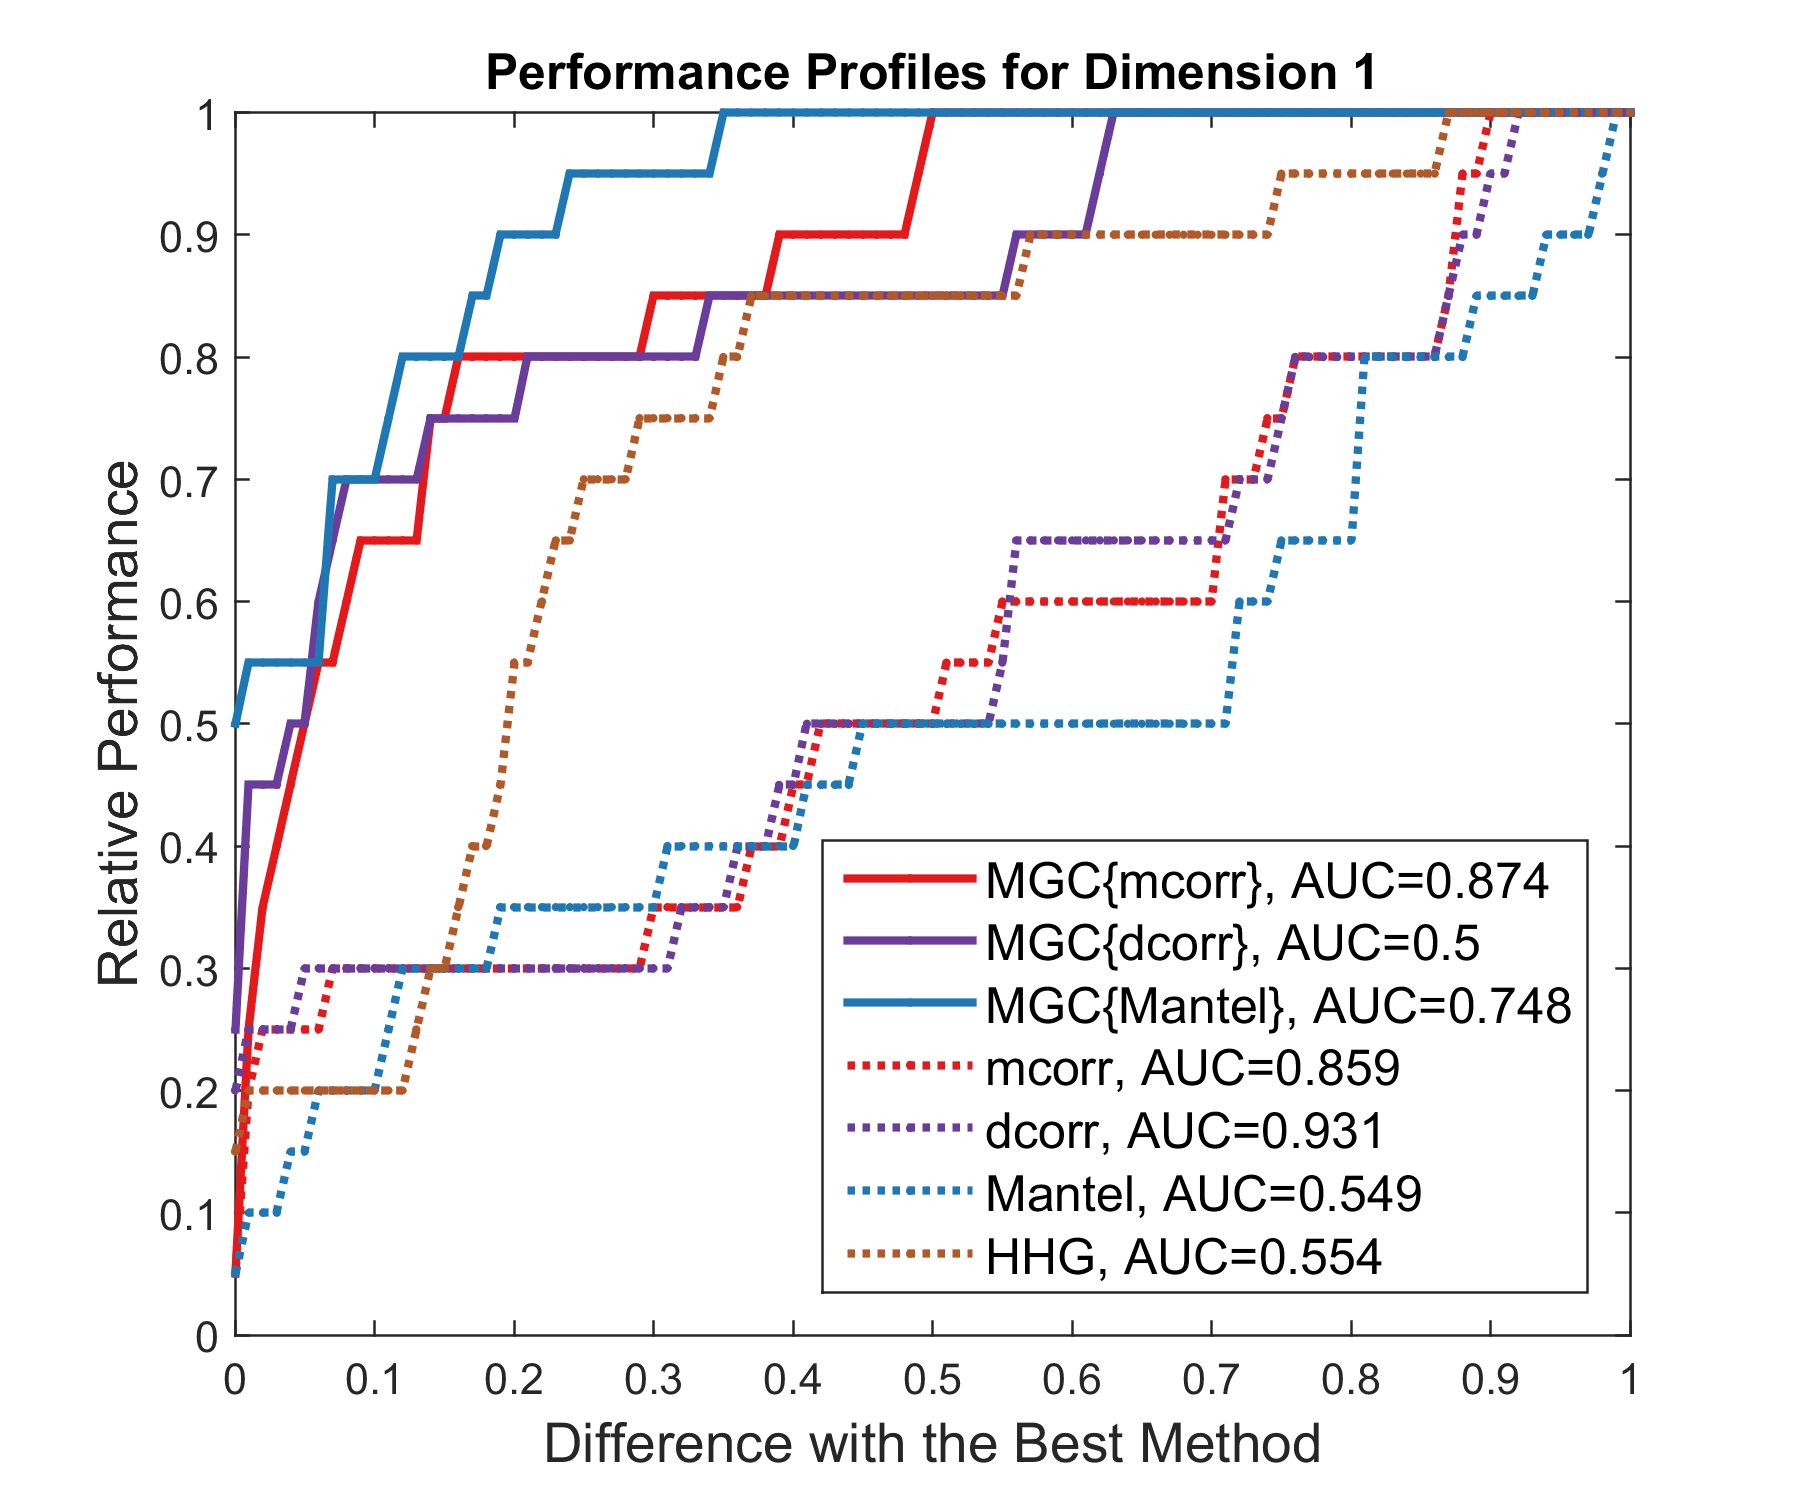
\includegraphics[width=0.5\textwidth]{../Figures/Fig3b}
}
\hfil
\subfloat[]{
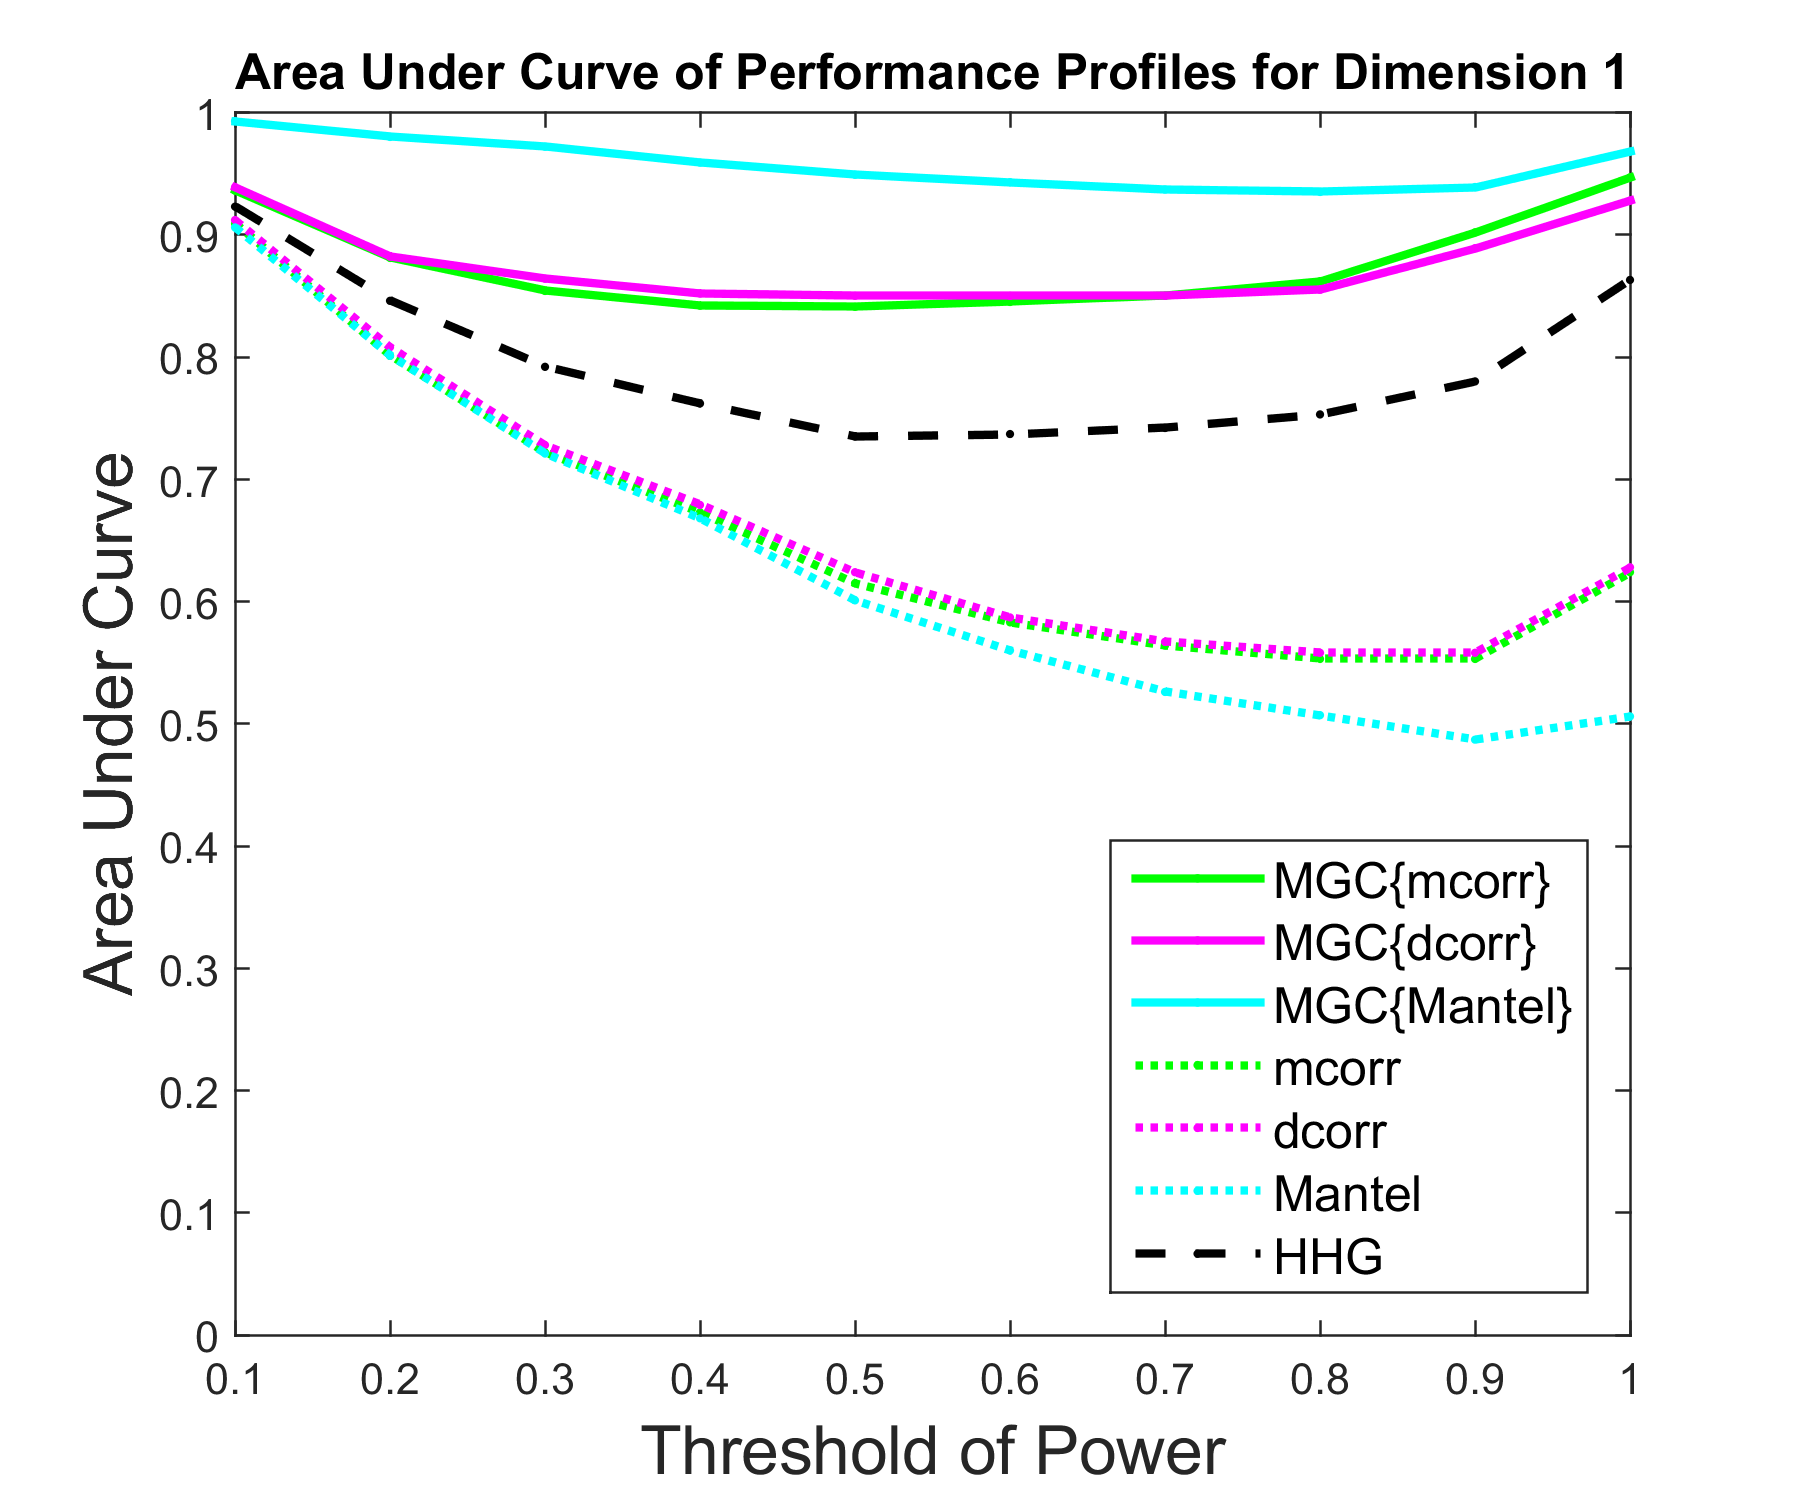
\includegraphics[width=0.5\textwidth]{../Figures/Fig4b}
}
\hfil
\subfloat[]{
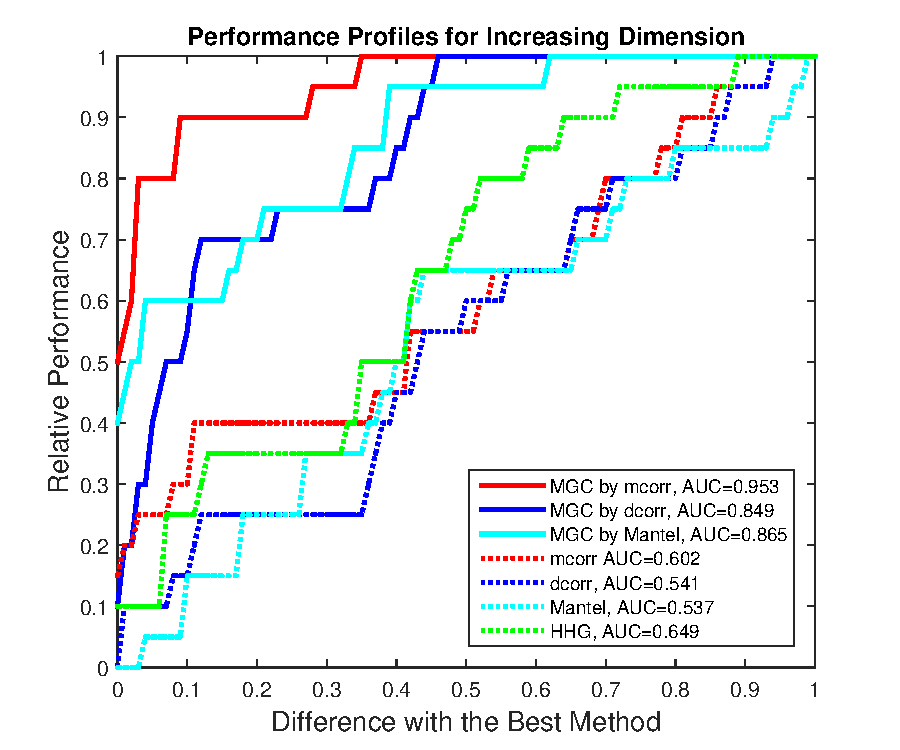
\includegraphics[width=0.5\textwidth]{../Figures/Fig7b}
}
\hfil
\subfloat[]{
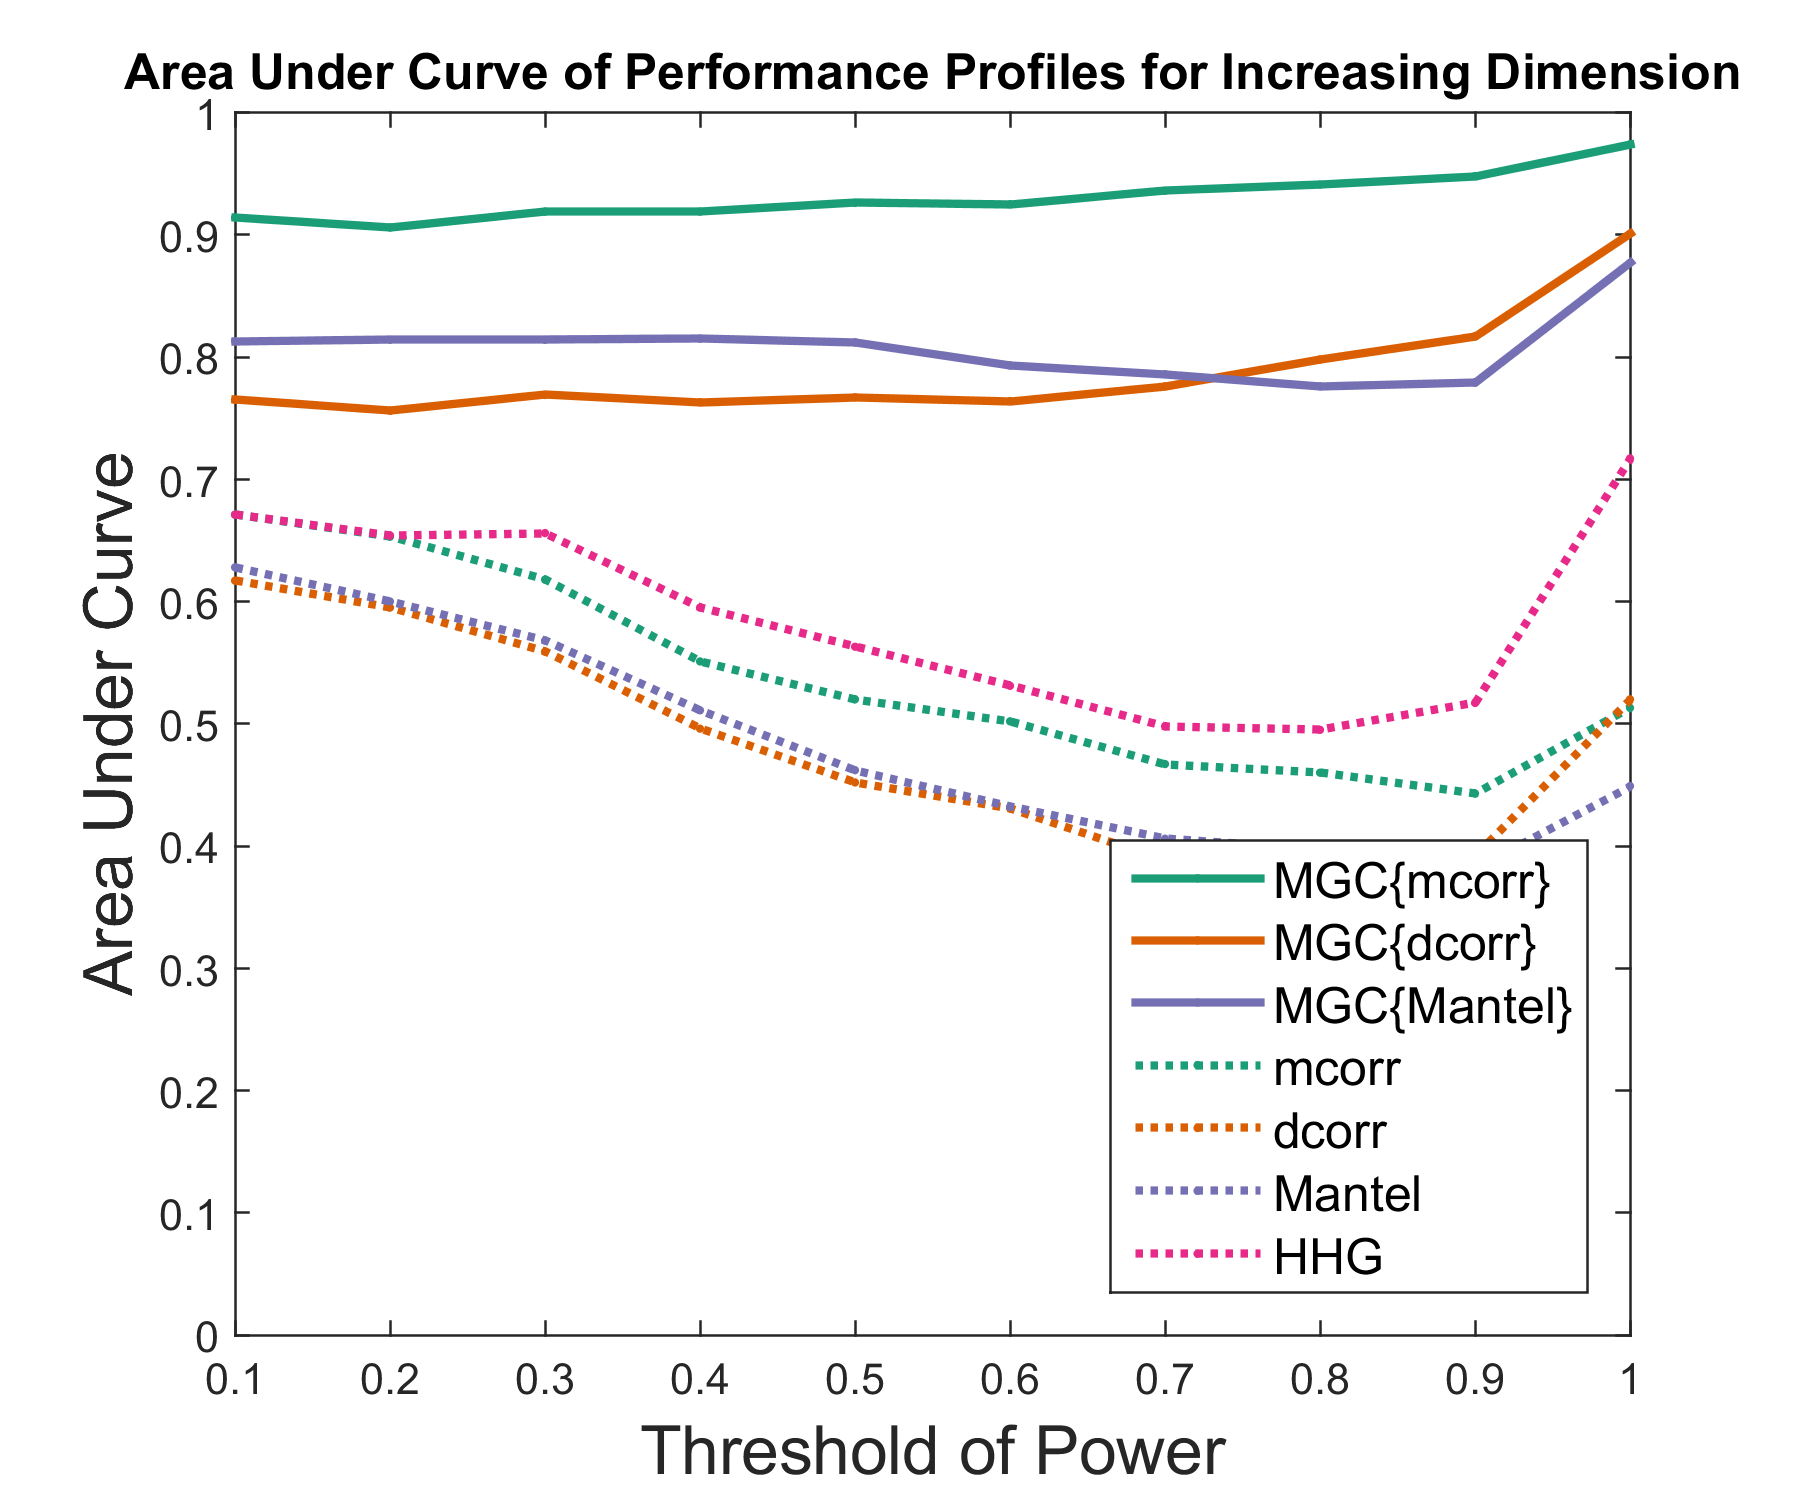
\includegraphics[width=0.5\textwidth]{../Figures/Fig8b}
}
\caption{Same Figures as Figure~\ref{fig:pp}, adding in LGC by dcorr and LGC by Mantel}
\label{fig:pp2}
\end{figure}

\section{Data Collection}



\section{Performance Profiles}

The performance profiles are drawn by the following steps:

Suppose there are $S$ methods and $T$ different problems, and we denote the respective powers as $\beta_{\alpha}^{t}(s)$ for $s=1,\ldots,S$ and $t=1,\ldots,T$ at a fixed type 1 error $\alpha$. Then the relative performance for each method is defined as follows:
\begin{align*}
performance_{s}(x) &= \frac{1}{T} \sum_{t=1}^{T} I((\beta_{\alpha}^{t}(*)-\beta_{\alpha}^{t}(s)) \leq x)
\end{align*}
where $x \in [0,1]$ and $\beta_{\alpha}^{t}(*) =\max_{s} \beta_{\alpha}^{t}(s)$ denotes the best testing power in the $t$th problem. Namely $x$ stands for the difference with respect to the best power, and the relative performance of each method equals the proportion of simulations that the method is worse than the best method by no more than $x$. For example, at $x=0.1$, LGC has a relative performance of $0.75$ if and only if there are $15$ out of $20$ simulations that LGC is worse than the best method by no more than $0.1$ in testing power. 

Note that the performance profiles at $x=0$ stands for the proportion of simulations that the method has the best power; and the curve always increases to $1$ at $x=1$. 

\section{Dependence Measures}
\label{main}

XXX I like the following notations:

$x_i \in \mc{X} \subset \Real^{d_x}$, $\mb{x} \sim F_x$, and $X=\{x_1,\ldots,x_n\}$ and similarly for $\mb{y}$. then $A=(a_{ij})$. 

so, lower case for scalars, caps for vectors and matrices, bold for random variables, and script for spaces.  

i'd let the centered distances be denote $A^H$ and the modified ones $A^M$.
and the local ones $\mt{A}$.

you sometimes write $A_{ij}$ to mean the scalar (un-center and normalized distance), which i think is confusing. i realize the standard is confusing.

i'm open to other consistent conventions.
XXX

YYY
I have adopted most of the above notations, except: I used $f_{x}$ for distribution rather than $F_{x}$; and $C/C^{H}/C^{M}$ to denote the distances, doubly centered distance, modified distance (rather than $A/A^{H}/A^{M}$), so they do not conflict with your notation of $a_{ij}$ in the equation of general correlation coefficient, but I can change them if necessary.
YYY

In this section, we review the Mantel test, distance correlation, modified distance correlation, and the HHG test in order.

\subsection{(Global) Mantel Test}
\label{sec:mantel}
For Mantel/dcorr/mcorr, they all start with two Euclidean distance matrices $C=(c_{ij}), D=(d_{ij}) \in \Real^{n \times n}$, where $c_{ij}=\|x_{i}-x_{j}\|_{2}$ and $d_{ij}=\|y_{i}-y_{j}\|_{2}$. 

Then the Mantel coefficient \cite{Mantel1967} is defined as 
\begin{equation}
Mantel(X,Y)=\frac{\sum_{i \neq j}^{n}(c_{ij}-\hat{E}(C))(D_{ij}-\hat{E}(D))}{\sqrt{\sum_{i \neq j}^{n}(c_{ij}-\hat{E}(C))^2 \sum_{i \neq j}^{n}(d_{ij}-\hat{E}(D))^2}},
\end{equation}
where $\hat{E}(C)=\frac{1}{n(n-1)}\sum_{i \neq j}^{n}(c_{ij})$ and similarly for $\hat{E}(D)$. In terms of the general correlation coefficient in Equation~\ref{generalCoef}, the Mantel coefficient essentially takes $a_{ij}=c_{ij}-\hat{E}(C)$ and $b_{ij}=d_{ij}-\hat{E}(D)$ when $i \neq j$, and $a_{jj}=b_{jj}=0$.

Therefore, the Mantel coefficient treats the two distance matrices as two observation vectors and calculates the Pearson's product-moment correlation coefficient between them. Then the Mantel test is carried out by the permutation test.

Unlike distance correlation and HHG, the Mantel test is not consistent against all dependent alternatives; but it has been a very popular method in biology and ecology due to its simplicity. Indeed we can observe from Figure~\ref{fig:D2} that the global Mantel coefficient is sub-optimal and appears to be not consistent for many dependencies; but local graph correlation implemented by Mantel nevertheless achieves comparable performances as other variants of LGC, which implies that LGC by Mantel may be consistent against most, if not all dependent alternatives.

\subsection{(Global) Distance Correlation}
\label{main1}
Starting with the two Euclidean distance matrices $C$ and $D$ for $X$ and $Y$, the sample distance covariance is defined on the doubly centered distance matrices $C^{H}$ and $D^{H}$:
\begin{equation}
\label{dcovEqu}
dcov(X,Y)=\frac{1}{n^2}\sum_{i,j=1}^{n}c^{H}_{ij}d^{H}_{ij},
\end{equation}
where $C^{H}=HCH$, $D^{H}=HDH$ with $H=I_{n}-\frac{J_{n}}{n}$. Then the sample distance variance is defined as
\begin{align*}
dvar(X) &=\frac{1}{n^2}\sum_{i,j=1}^{n}c^{H}_{ij}d^{H}_{ij}\\
dvar(Y) &=\frac{1}{n^2}\sum_{i,j=1}^{n}c^{H}_{ij}d^{H}_{ij},
\end{align*}
and the sample distance correlation follows as
\begin{equation}
\label{dcorrEqu}
dcorr(X,Y)=\frac{dcov(X)}{\sqrt{dvar(X) \cdot dvar(Y)}}.
\end{equation}
In the form of the general correlation coefficient in Equation~\ref{generalCoef}, distance correlation takes $a_{ij}=c^{H}_{ij}$ and $b_{ij}=d^{H}_{ij}$ for all $i,j$.

It is shown in \cite{SzekelyRizzoBakirov2007} that as $n \rightarrow \infty$, $dcorr(X,Y) \rightarrow dcorr(\mb{x},\mb{y}) \geq 0$, where $dcorr(\mb{x},\mb{y})$ denotes the population distance correlation between the random variables $\mb{x}$ and $\mb{y}$. The population distance correlation is defined by the characteristic functions, which is $0$ if and only if $\mb{x}$ and $\mb{y}$ are independent. Thus the sample distance correlation is a consistent test for independence, i.e., the testing power $\beta_{\alpha}(dcorr(X,Y))$ converges to $1$ as $n$ increases, at any fixed type $1$ error level $\alpha$. 

Note that the consistency result assumes finite second moments of $\mb{x}$ and $\mb{y}$; and the consistency holds for a family of metrics including the Euclidean distance \cite{Lyons2013}. Furthermore, all of $dcov, dvar, dcorr$ are always non-negative; and the $dcorr$ defined here is actually the square of distance correlation in \cite{SzekelyRizzoBakirov2007}, but for simplicity we drop the square naming here.

\subsection{(Global) Modified Distance Correlation}
\label{sec:gmd}
In case of high-dimensional data where the dimension $d_{x}$ or $d_{y}$ increases with the sample size $n$, the distance correlation $dcorr$ may no longer be appropriate. For example, even for independent Gaussian distributions, $dcorr(X,Y) \rightarrow 1$ as $d_{x}, d_{y} \rightarrow \infty$, which may severally impair the testing power of dcorr in high dimension simulations.

To tackle this problem, the modified distance correlation is proposed in \cite{SzekelyRizzo2013a}. The modified distance covariance is defined as
\begin{equation}
\label{mcovEqu}
mcov(X,Y)=\frac{n}{(n-1)^2(n-3)}(\sum_{i \neq j}^{n}c^{M}_{ij}d^{M}_{ij}-\frac{2}{n-2}\sum_{j=1}^{n}c^{M}_{jj}d^{M}_{jj}),
\end{equation}
where $C^{M}$ modifies the entries of $C^{H}$ by
\[c^{M}_{ij} = \left\{
  \begin{array}{lr}
    c^{H}_{ij}-\frac{c_{ij}}{n}, & \mbox{ if } i \neq j \\
    \frac{n\sum_{i}c_{ij}-\sum_{i,j}c_{ij}}{n^2}, &\mbox{ if } i = j 
  \end{array}
\right.
\]
and similarly for $D^{M}$. Then $mvar(X)$ can be defined by replacing all $d^{M}_{ij}$ in Equation~\eqref{mcovEqu} by $c^{M}_{ij}$, similarly for $mvar(Y)$. 

If $mvar(X) \cdot mvar(Y) \leq 0$, the modified distance correlation is set to $0$ (negativity can only occur when $n\leq 2$, equality can only happen in very special cases); otherwise it is defined as
\begin{equation}
\label{mcorrEqu}
mcorr(X,Y)=\frac{mcov(X,Y)}{\sqrt{mvar(X) \cdot mvar(Y)}}.
\end{equation}
In the form of the general correlation coefficient, modified distance correlation takes $a_{ij}=c^{M}_{ij}$ and $b_{ij}=d^{M}_{ij}$ for $i \neq j$, and $a_{jj}=\sqrt{-\frac{2}{n-2}}c^{M}_{jj}$ and $b_{jj}=\sqrt{-\frac{2}{n-2}}d^{M}_{jj}$. Note that since the diagonals are complex numbers, we will tweak them (without changing its theoretical consistency) when we implement local graph correlation by mcorr, see in Section~\ref{main2}.

It is shown in \cite{SzekelyRizzo2013a} that $mcorr(X,Y)$ is an unbiased estimator of the population distance correlation $dcorr(\mb{x},\mb{y})$ for all $d_{x}, d_{y}, n$; and $mcorr$ is approximately normal even if $d_{x},d_{y} \rightarrow \infty$. Thus it is also a consistent test of independence, but may work better than dcorr under high-dimension dependencies. 

%To summarize dcorr and mcorr, both methods are great for testing independence of Euclidean data due to their theoretical consistency, with the modified test statistic being more superior under high-dimensional dependency; and it is a flourishing concept by a series of papers \cite{BakirovRizzoSzekely2006, SzekelyRizzoBakirov2007, SzekelyRizzo2009, BickelXu2009, Kosorok2009, Remillard2009, LiZhongZhu2012, Lyons2013, SzekelyRizzo2013a, SzekelyRizzo2013b, SzekelyRizzo2014}. However, the required sample size for achieving a good testing power very much depends on the type of dependency underlying the given data, e.g. for perfect linear relationship, distance correlation usually requires less than $10$ points for a permutation test to declare significance; but for some nonlinear relationships like circle, distance correlation yields no significance even at $n=100$. Because real data rarely exhibits perfect linear relationship, and in practice large amount of data may not always be available, a better finite-sample method is of tremendous value: it not only yields a better testing power for the same sample size, but may also requires much less sample data for the permutation test to declare significance, which in turn saves the running time and data collection process. 

\subsection{Heller, Heller \& Gorfine (HHG)}
\label{sec:hhg}
Like dcorr and mcorr, the HHG test in \cite{HellerGorfine2013} is also distance-based and consistent; and like our local graph correlation, it makes use of the rank information, but in a different manner. It applies Pearson's chi-square test to ranks of distances within each column, and is shown to be better than many global tests including dcorr under many common nonlinear dependencies in \cite{GorfineHellerHeller2012, HellerGorfine2013}. 

Defining 
\begin{align*}
H_{11}(i,j) &= \sum_{q=1,q\neq i,j}^{n}I(a_{ik} \leq a_{ij})I(b_{ik} \leq b_{ij}) \\
H_{12}(i,j) &= \sum_{q=1,q\neq i,j}^{n}I(a_{ik} \leq a_{ij})I(b_{ik} > b_{ij}) \\
H_{21}(i,j) &= \sum_{q=1,q\neq i,j}^{n}I(a_{ik} > a_{ij})I(b_{ik} \leq b_{ij}) \\
H_{22}(i,j) &= \sum_{q=1,q\neq i,j}^{n}I(a_{ik} > a_{ij})I(b_{ik} > b_{ij}),
\end{align*}
the HHG test statistic is then
\begin{align*}
HHG(X,Y) &= \sum_{i=1,j\neq i}^{n} \frac{(n-2)(H_{12}(i,j)H_{21}(i,j)-H_{11}(i,j)H_{22}(i,j))^2}{H_{1 \cdot}(i,j)H_{2 \cdot}(i,j)-H_{\cdot 1}(i,j)H_{\cdot 2}(i,j)},
\end{align*}
where $H_{1 \cdot}=H_{11}+H_{12}$ and similarly for others.

It is clear that the HHG statistic is structurally different from Mantel/dcorr/mcorr, and cannot be expressed in terms of the general correlation coefficient in Equation~\ref{generalCoef}. Thus local graph correlation is not directly applicable to HHG.

In our numerical simulations HHG seems to fall a bit short when testing against high-dimensional or close to linear dependencies, but is otherwise a strong competitor and more advantageous than all other global tests under most nonlinear dependencies. %However, local graph correlation is able to approximate or surpass its performances in most cases.

\section{Local Graph Correlation}
\label{main2}

For any test statistic that can be expressed by the general correlation coefficient in Equation~\ref{generalCoef}, its local graph correlation coefficient can be implemented by Equation~\ref{localCoef}. As an example, we show how local graph correlation is implemented by modified distance correlation here; and explain some implementation issues.

By section~\ref{sec:gmd}, modified distance correlation is equivalent to the general correlation coefficient by taking $a_{ij}=c^{M}_{ij}$ and $b_{ij}=d^{M}_{ij}$ for $i \neq j$, and $a_{jj}=\sqrt{-\frac{2}{n-2}}c^{M}_{jj}$ and $b_{jj}=\sqrt{-\frac{2}{n-2}}d^{M}_{jj}$. But if we implement local graph correlation by mcorr directly based on Equation~\ref{localCoef}, $g_{kl}$ may be a complex number when ties occur, e.g., $rank(a_{ij})=0$ and $rank(b_{ij})>0$.

Note that $a_{jj}$ and $b_{jj}$ converge to $0$, and the expectations of $c^{M}_{jj}$ and $d^{M}_{jj}$ are also $0$. Therefore, instead of using complex number diagonals, we can let $a_{jj}=b_{jj}=0$ with little inferential impact. Then the local version of modified distance covariance becomes
\begin{align*}
mcov_{kl}(X,Y) = \frac{n}{(n-1)^2(n-3)}(\sum_{i \neq j}^{n}c^{M}_{ij}d^{M}_{ij}I(0<rank(a_{ij})<k))I(0<rank(b_{ij})<l),
\end{align*}
similarly for $mvar_{k}$, and eventually $mcorr_{kl}$ as the local test statistic of mcorr. After the above tweak to the diagonals, LGC by mcorr maintains its consistency, has little performance difference from before, and is still superior under high-dimensional dependencies.

There exists another problem for ties, which is of particular importance for LGC by mcorr: modified distance correlation improves over the original distance correlation, mostly because its adjustment to the diagonal terms; and if there are repeating points in the data, it is necessary to adjust them in the same manner as the diagonal terms, or mcorr will lose its advantage and not function properly in a permutation test. Although repeating data happen with probability $0$ for data generated by continuous distribution, it can happen for discrete distribution and during resampling.

The tie problem is handled by taking minimal rank among ties, and let $a_{ij}$ equal $a_{jj}$ whenever $x_{i}=x_{j}$ (or any $x_{i}$ that is rank zero) in Equation~\ref{localCoef}. This is necessary for any global correlation coefficient that $a_{jj}$ can be different from $a_{ij}$ when $x_{i}=x_{j}$, such as Mantel or mcorr; but does not matter for dcorr, for which $a_{jj}=a_{ij}$ always holds when $x_{i}=x_{j}$. As long as $a_{ij}$ is handled properly when $x_{i}=x_{j}$, in practice one can break the ties randomly or use average ranks.

Last but not least, in the local family of tests it suffices to exclude $g_{1l}$ and $g_{k1}$, because it holds that $g_{1l}=g_{k1}=g_{11}$, which does not consider any neighbor, merely counts the diagonal terms in the distance matrices, and not meaningful for testing independence. Therefore they are not considered in our main algorithm.

\section{Testing Procedure}
\label{main3}

In this subsection we elaborate on the testing procedure by local graph correlation.

\subsection{LGC Algorithm}

For two given data $X$ and $Y$, the following bootstrap-based algorithm returns the p-value of LGC in the permutation test: it estimates the optimal neighborhood choice by bootstrap, then returns the p-value of the estimated optimal local test from a random permutation test.

\begin{algorithm}
\label{alg1}
%\caption{Local Graph Correlation Testing Algorithm} 
\begin{algorithmic} 
\State \textbf{Input}: Two data sets $X$ and $Y$ of the same sample size $n$, but possibly different dimensions or spaces (e.g., shapes and graphs). A pre-defined significance level $\alpha$, a parameter $r$ used for number of random replicates, and a global test statistic $g_{nn}$ that can be expressed by Equation~\ref{generalCoef}. 

\State 1. \textbf{Distance transformation}:

Transform $X$ and $Y$ into two $n \times n$ distance matrices $C$ and $D$. 

\State 2. \textbf{Estimate the optimal neighborhood of LGC by bootstrap}:

First we generate a random resampling of size $n$, apply the same resampling to both $X$ and $Y$, and denote the re-sampled data as $X^{'}$ and $Y^{'}$. Then calculate $g_{kl}(X^{'}, Y^{'})$ for all $k,l=2,\ldots,n$ by Equation~\eqref{localCoef}. 

We further generate a random permutation matrix $Q$, and calculate $g_{kl}(X^{'}, Y^{'}Q)$ for all $k,l=2,\ldots,n$. (Alternatively, we can resample again to give an independent $Y^{''}$, and calculate $g_{kl}(X^{'}, Y^{''})$ instead.)

Repeat the above procedure for $r$ independent replicates, which yields the empirical distributions of $g_{kl}$ under the alternative and under the null respectively. 

Then we can estimate the testing power of all local tests at the type 1 error level $\alpha$ from their empirical distributions. Denote the estimated powers as $\hat{\beta}_{\alpha}(g_{kl})$, we pick the optimal neighborhood choice that maximizes the power:
\begin{equation}
\label{power}
(k^{*},l^{*})=\arg\max_{k,l}\{\hat{\beta}_{\alpha}(g_{kl}), k,l\in [2,\ldots,n]\},
\end{equation}

\State 3. \textbf{Calculate the p-value of local graph correlation by permutation test}: 

Calculate the observed statistic $g_{k^{*}l^{*}}(X, Y)$, and compare to the permuted statistic as follows:
\begin{equation}
\label{pvalue}
p=Prob(g_{k^{*}l^{*}}(X, Y)>g_{k^{*}l^{*}}(X, YQ)),
\end{equation}
where $Q$ denotes a random permutation of size $n$. Since it is usually infeasible to consider all possible permutations, the p-value is estimated by randomly generating $r$ permutations.

If there are more than one optimal neighborhood choice, use the mean p-value.

\State \textbf{Output}: The p-value of LGC; reject the null hypothesis of independence if and only if the p-value of LGC is less than the significance level $\alpha$.
\end{algorithmic} 
\end{algorithm} 

This is the algorithm used in the real data experiment for the p-value of LGC, and in fact the p-values of all global tests, except that the global tests do not need the neighborhood estimation step (where they essentially take $k^{*}=l^{*}=n$).

Note that the algorithm can start with two distance matrices $C$ and $D$ directly rather than the Euclidean data, although theoretical consistency may not hold for arbitrary metrics.

\subsection{Evaluation by Simulations}

For data of known distributions, the statistical powers of any test can be directly estimated by Monte-Carlo replicates as follows:

When the true joint distribution $f_{xy}$ is known, we can directly generate $X$ and $Y$ using $f_{xy}$, and estimate the empirical distributions of $g_{kl}(X,Y)$ under the alternative by repeatedly generating the dependent data for $r$ Monte-Carlo replicates. Then we can also generate $Y^{'}$ independently from the marginal distribution, and estimate the empirical distributions of $g_{kl}(X,Y^{'})$ under the null.

From the above empirical distributions, we estimate the testing power of $g_{kl}$ at type 1 error level $\alpha$ as follows: for each $k,l$, denote the empirical distribution $g_{kl}$ under the null and the alternative as $\hat{F}_{kl}^{N}$ and $\hat{F}_{kl}^A$ respectively; calculate the critical value $\hat{\mu}_{kl}$ by $1-\alpha=Prob(\hat{F}_{kl}^{N}<\hat{\mu}_{kl})$, and obtain the power by $\beta_{\alpha}(g_{kl})=Prob(\hat{F}_{kl}^{A}>\hat{\mu}_{kl})$; at last take the maximal power $\hat{\beta}_{\alpha}(g)=\max{\hat{\beta}_{\alpha}(g_{kl}), k,l=2, \ldots,n}$ as the empirical power of LGC.

XXX please clarify in the above ``how'' you get power from those two distributions. XXX
YYY is the above clear to you now?  YYY

We call the above evaluation procedure as the independence test, which approximates the bootstrap procedure in step 2 of the algorithm. Similarly, we can evaluate dcorr, mcorr, HHG, and the Mantel coefficient by the independence test, by replacing $g_{kl}$ with the respective $g_{nn}$. 

It is faster to derive the testing power by the independence test than the permutation test in the main algorithm; in fact, if the true distribution is known, the independence test is also the best way to estimate the optimal neighborhood choice of LGC, and step $2$ of our main algorithm is an approximation of the independence test. 

As long as the empirical distribution of the resampled data is sufficiently close to the true distribution for sufficiently large $r$, the power of any test based on the independence test should approximate its testing power from the permutation test; and the optimal neighborhood of LGC estimated from the bootstrap procedure should be close to true optimal.

Therefore, for the known distributions in the simulations, we report the empirical testing powers by the independence test. A consistent test should have its power converging to $1$ under any type of dependency, and has power equals the type $1$ error $\alpha$ in the absence of dependency.  

\section{Proofs}
\label{sec:pfs}
%Although distance correlation is already consistent against all alternatives, it may not always yield a good finite-sample testing power for a particular dependency type; while our local graph correlation is able to improve the testing power by choosing the best neighborhood for a given joint distribution. 

%The advantage of using k-nearest-neighbor in distance matrices, lies in its capability to exclude the product of small distances in one data set and large distances in the other data set: after double centering, the centered small distance is usually negative and the centered large distance is usually positive, and including such product reduces the magnitude of local distance covariance under the alternative. While excluding such product by k-nearest-neighbor can increase the magnitude of local distance covariance under the alternative, albeit at the cost of increasing its magnitude under the null as well. 

\begin{thm}
Suppose for given $f_{xy}$ and $\alpha$, $\beta_{\alpha}(g_{nn}) \rightarrow 1$ as $n \rightarrow \infty$ for given $f_{xy}$ and $\alpha$, then $\beta_{\alpha}(g) \rightarrow 1$ as well.

Therefore, local graph correlation is consistent against all dependent alternatives of finite second moments, when it is built on distance correlation or modified distance correlation.
\end{thm}
\begin{proof}
The power of local graph correlation satisfies
\begin{equation}
\beta_{\alpha}(g)=\max_{k,l}\{\beta_{\alpha}(g_{kl}), k,l\in [2,\ldots,n]\} \geq \beta_{\alpha}(g_{nn}).
\end{equation}
So if $\beta_{\alpha}(g_{nn}) \rightarrow 1$, we also have $\beta_{\alpha}(g) \rightarrow 1$.

Since dcorr and mcorr are consistent against all alternatives of finite second moments by \cite{SzekelyRizzoBakirov2007, SzekelyRizzo2013a}, clearly their local graph correlation are also consistent.
\end{proof}

\begin{thm}
Suppose $\mb{y}=c\mb{x}$ for a non-zero scalar $c$. Then for any $n$ and $\alpha$ it always holds that
\begin{equation}
\beta_{\alpha}(g) = \beta_{\alpha}(g_{nn}).
\end{equation}

Thus local graph correlation is equivalent to the global correlation coefficient under linear dependency.
\end{thm}
\begin{proof}
To show that LGC is no better than its global correlation coefficient, it suffices to show the p-value of $g_{kl}$ is always no less than the p-value of $g_{nn}$ for all $k,l$.

%Let us first suppose $\mb{x}$ is continuously distributed, such that with probability $1$ no two columns of $X$ have the same magnitude.

Under linear dependency, for any global correlation coefficient satisfying Equation~\ref{generalCoef}, by Cauchy-Schwarz inequality we have
\begin{equation}
1=g_{nn}(X, Y) \geq g_{nn}(X, YQ)
\end{equation}
for any permutation matrix $Q$, for which the equality holds if and only if $X$ is a scalar multiple of $YQ$. It follows that the p-value of $g_{nn}$ is $\frac{|\Omega|}{n!}$, where $|\Omega|$ equals the cardinality of $\Omega=\{Q, X \mbox{ is a scalar multiple of }YQ\} \subset \{\mbox{all possible permutation matrices }Q\}$. Since the identity matrix is an element of $\Omega$, the p-value of $g_{nn}$ is at least $\frac{1}{n!}$.

For any $Q \in \Omega$ and any $k,l$, clearly $g_{kl}(X,Y)=g_{kl}(X,YQ)$. It follows that the p-value of $g_{kl}$ is no less than $\frac{|\Omega|}{n!}$; and there may exist other permutation matrices $Q \notin \Omega$ such that $g_{kl}(X,Y) \leq g_{kl}(X,YQ)$. Thus the p-value of $g_{kl}$ is always bounded below by the p-value of $g_{nn}$.

Therefore for any $k,l$, we must have $\beta_{\alpha}(g_{kl}) \leq \beta_{\alpha}(g_{nn})$. Since local graph correlation includes the global test statistic, it follows that $\beta_{\alpha}(g) = \beta_{\alpha}(g_{nn})$ at any given type $1$ error level $\alpha$.

Note that this theorem holds for LGC based on any of mcorr/dcorr/Mantel, and in fact LGC by any general correlation coefficient that can be expressed by Equation~\ref{generalCoef}.
\end{proof}

\begin{thm}
There exists $f_{xy}$, $n$ and $\alpha$ such that 
\begin{equation}
\beta_{\alpha}(g) > \beta_{\alpha}(g_{nn}).
\end{equation}

Thus local graph correlation can be better than its global counterpart under certain nonlinear dependency.
\end{thm}
\begin{proof}
We give a simple discrete example of $f_{xy}$ at $n=7$ such that the p-value of $g_{kl}$ for $(k,l) \neq (n,n)$ is always lower than the p-value of $g_{nn}$, which is equivalent to say the permutation test power $\beta_{\alpha}(g)$ is larger than $\beta_{\alpha}(g_{nn})$ at an appropriate type $1$ error level $\alpha$.

Suppose under the alternative, $f_{xy}$ is distributed as follows:
\begin{align*} 
\mb{x} &\in \{-1,-\frac{2}{3},-\frac{1}{3},0,\frac{1}{3},\frac{2}{3},1\} \mbox{ without replacement}, \\
\mb{y} &= \mb{x}^2,
\end{align*}
which is a discrete version of the quadratic relationship in the simulations.

In this example we can easily consider all possibilities of $C^{M}$ and $D^{M}$, and calculate $g_{kl}(X, Y)$ and $\{g_{kl}(X, YQ)\}$ for all permutation matrices $Q$. Take $g_{nn}=mcorr, n=l=7, k=2$ as an example, $g_{nn}(X, Y)=0.0783$, $g_{kl}(X, Y)=0.0583$, and similarly all possible permuted test statistics. It follows that the p-value of $g_{nn}$ is $0.2683$, while the p-value of $g_{kl}$ is $0.1571$. 

Therefore we have an example of $f_{xy}$ and $n$ such that $\beta_{\alpha}(g_{kl}) > \beta_{\alpha}(g_{nn})$ for some $(k,l) \neq (n,n)$: by choosing $\alpha=0.2, n=7$, we have $1=\beta_{\alpha}(g_{kl}) > \beta_{\alpha}(g_{nn})=0$ at $(k,l)=(2,7)$. Then $\beta_{\alpha}(g)=\max_{k,l}{\beta_{\alpha}(g_{kl})}=1>\beta_{\alpha}(g_{nn})$, and LGC by mcorr is better than the global mcorr.

Note that we can always consider equally spaced sample points (or randomly sampled points) in $[-1,1]$ for $X$, increase $n$ and reach the same conclusion with smaller p-values; but the computation of all possible permuted test statistics becomes much more time-consuming as $n$ increases. Furthermore, the same conclusion holds for LGC based on dcorr or Mantel using the same example.
\end{proof}


\bibliographystyle{alpha}
\bibliography{references}

\end{document}